\section{Auswertung}

\subsection{Radkasten}

Im folgenden Kapitel werden auf Basis der in \ref{sub:method_wheelcase} eingeführten Methodik Experimente durchgeführt.
Es wird so vorgegangen, dass zuerst ein eher einfaches Experiment durchgeführt wird, auf dessen Basis die grundsätzlichen Annahmen über das Problem der Radkastenoptimierung geprüft werden können.
Darauf aufbauend werden aufwendigere und ausführlichere Experimente durchgeführt, um für die Realität nutzbare Ergebnisse zu erhalten.

\subsubsection{Initiales Validierungsexperiment}
\label{sub:exp1st}
\begin{table}[h]
	\centering
	\begin{tabularx}{.75\textwidth}{ll}\hline
		Anzahl initialer Samples & 100 \\
		Anzahl Samples & 500 \\
		Anzahl neuer Samples pro Akquiseschleife & 20 \\
		Anzahl Generationen Akquise-MAP-Elites & 1024 \\
		Kinder pro Generation Akquise-MAP-Elites & 32 \\
		Anzahl Generationen Ergebnis-MAP-Elites & 2048 \\
		Kinder pro Generation Akquise-MAP-Elites & 32 \\
		Auflösung der MAP-Elites Karte & 25 * 25  \\
		\hline
		Freiheitsgrade & 6 \\
		Mittelwertgewichtung & 1 \\
		Varianzgewichtung & 2 \\
		Constraintgewichtung & 1 \\
	\end{tabularx}
	\caption{Parametrisierung des ersten Experiments}
	\label{tab:param1st}
\end{table}

Das Primärziel des ersten Experiments bestand darin zu verifizieren, dass der Algorithmus trotz Einbindung des Constraints korrekt funktioniert, d.~h. auch mit Constraint vergleichbare Werte bezüglich Luftwiderstandskoeffizienten erreicht werden, und der Algorithmus trotz des Constraints korrekt lernt.
Deshalb wurde die Parametrisierung vergleichsweise einfach gewählt, FFD-Deformationen fanden in zwei Punkten, in jeweils drei Richtungen statt.
\begin{figure}[h]
	\centering
	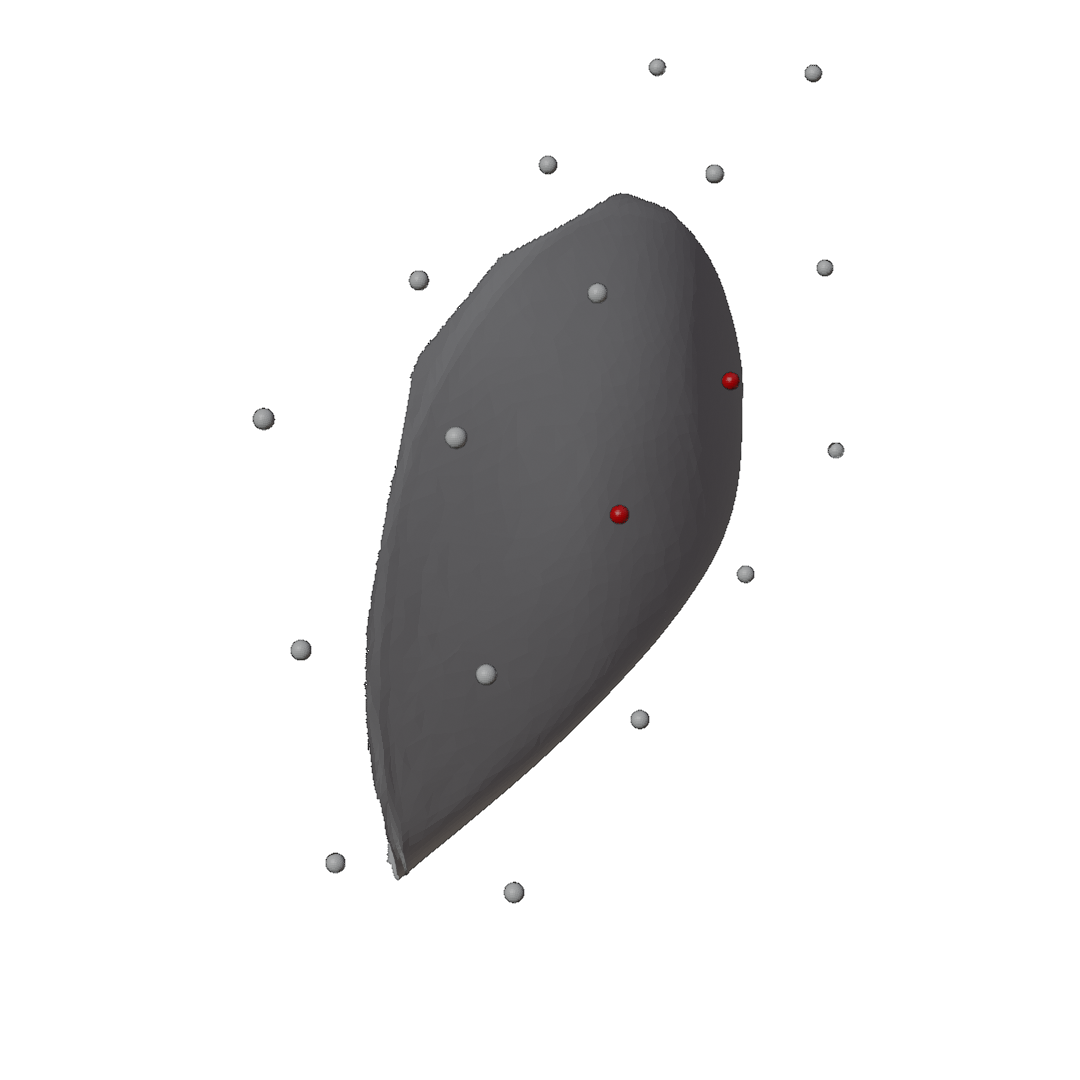
\includegraphics[width=.7\linewidth]{bilder/2ptDeformationPoints}
	\caption{Deformationspunkte des ersten Experiments}
	\label{fig:ffd1st}
\end{figure}
Auch wurde die Laufzeit so weit beschränkt, dass sinnvolle Aussagen darüber getroffen werden können, ob und wie gut der Algorithmus lernt, für finale Ergebnisse hingegen wäre die Anzahl an Samples die ausgewertet werden sowie die Anzahl an Genrationen für Akquise, und finaler Auswertung höher zu wählen.
Um bewerten zu können, ob die Einbindung des Constraints einen Effekt auf den Algorithmus hat, und um diesen Effekt quantifizieren zu können wurde der Algorithmus unter den in Tabelle \cref{tab:param1st} beschriebenen Parametern sowohl mit Constraint als auch ohne Constraint durchgeführt. 
\begin{figure}[h]
	\centering
	\begin{minipage}{0.45\textwidth}
		\centering
		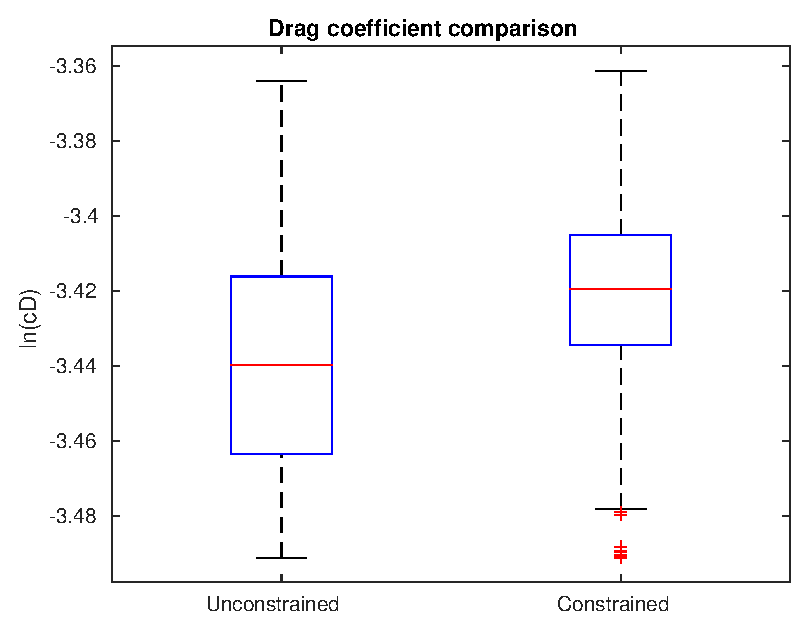
\includegraphics[width=1\linewidth]{bilder/2pt500Samples/dragBoxplot}
		\caption{Vergleich der Luftwiderstände der produzierten Lösungen}
		\label{fig:1stdragbox}
	\end{minipage}\hfill
	\begin{minipage}{0.45\textwidth}
		\centering
		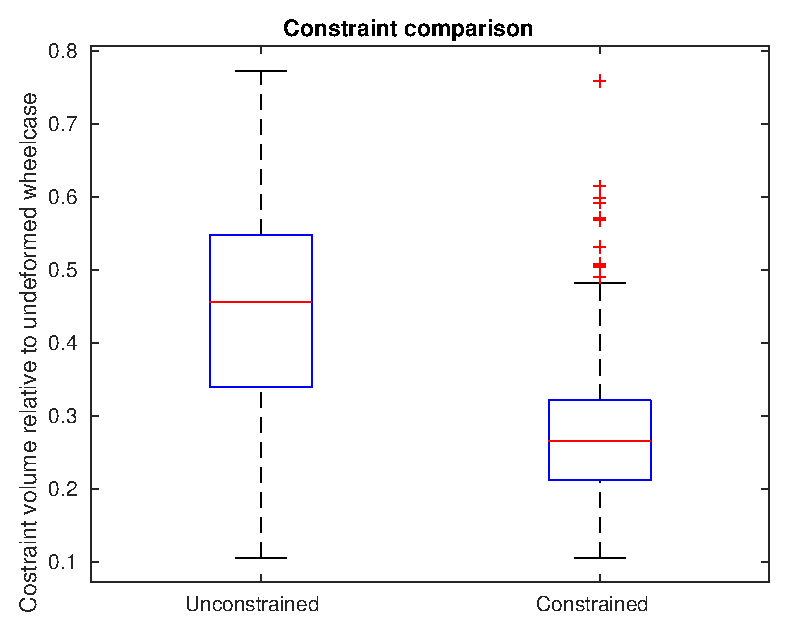
\includegraphics[width=1\linewidth]{bilder/2pt500Samples/constraintBoxplot}
		\caption{Vergleich der Constrainterfüllung der produzierten Lösungen}
		\label{fig:1stconbox}
	\end{minipage}
\end{figure}

Die Ergebnisse des ersten Experiments sehen vielversprechend aus in Abb. \cref{fig:1stdragbox} ist ein Vergleich der Luftwiderstandsergebnisse 
\footnote{Im Experiment wurde statt der direkten Luftwiderstandswerte, der natürliche Logarithmus dieser genutzt.} 
der erzeugten Lösungen abgebildet.
Die erste Beobachtung die gemacht werden kann ist, dass die produzierten Werte aus der Variante mit Constraint in der gleichen Größenordnung liegen wie die aus der Variante ohne Constraint.
Der Algorithmus scheint also auch mit Constraint noch korrekt zu lernen.
Es ist zu Erkennen, dass die Einbindung des Constraints zu einer Verschlechterung der Luftwiderstandswerte führt, eine Verschlechterung dieser durch eine Fokussierung auf zwei Ziele ist allerdings zu erwarten.
Trotzdem muss betont werden, dass die Verschlechterung erstaunlich klein ist, so beträgt der relative Unterschied zwischen dem Median der Version mit Constraint und dem Median der Version ohne nur \todo{genaue zahl}.

Um eine solche Verschlechterung zu rechtfertigen, sollte die Qualität des Sekundärziels herangezogen werden.
Dazu ist in \cref{fig:1stconbox} ein Vergleich bezüglich des Constraintvolumens dargestellt.
Die erste Beobachtung hier ist, dass die Einbindung des Constraints zu einer stärkeren Beachtung dessen führt.
Das ist offensichtlich das Ziel bei der Nutzung eines Constraints. 
Dass diese Erwartung erfüllt wird, zeigt, dass die Formulierung des Constraints in dieser Weise funktioniert.
Auch ist hervorzuheben, dass die relative Verbesserung des Constraints wesentlich stärker ist als die relative Verschlechterung des Luftwiderstands.
Eine Verschlechterung des Medians bezüglich des Luftwiderstands von \todo{genaue zahl} geht hier mit einer Verbesserung des Medians bezüglich des Constraints von \todo{genaue zahl} einher.

Interessant sind auch die Grenzen der Verteilungen, beide Verteilungen weisen eine untere Grenze von ca. $0,1$, sprich 10\% des Außenvolumens des nicht verformten Radkastens auf.
Dies lässt sich dadurch erklären, dass das Radausschlagsvolumen einen Teil unterhalb des Radkastens hat, der durch eine seitliche Deformation des Radkastens nicht eliminiert werden kann.
Die zweite interessante Grenze stellt die Obergrenze von $0,8$ dar.
Selbst die schlechteste Lösung in der Version ohne Constraint ist damit besser als der undeformierte Radkasten.
Dies kann einerseits an zu eng gewählten Deformationsparametern liegen, die genutzte Konfiguration erlaubte allerdings Deformationen nach innen.
Die plausiblere Hypothese ist, dass die Wahl der Breite des Radkastens als Feature bedeutet, dass eine Minimalbreite existiert, bei der nicht das Zentrum des Radkastens, sondern die Ränder den breitesten Punkt darstellen.
Jede Deformation die das Zentrum stärker nach innen verformt, würde in die gleiche Zelle der Karte eingeordnet werden.
Wenn weniger stark verformte Radkästen bezüglich deren Fitness optimaler sind, wird dies dazu führen, dass Radkästen mit einer stärkeren Verformung nach innen keinen Einzug in die Karte finden können.

Aufgrund der Tatsache, dass SAIL ein divergenter Optimierungsalgorithmus ist haben die finalen Verteilungen nur eingeschränkte Aussagekraft.
Besonders dadurch, dass das Feature der Breite des Velomobils mit der Schwierigkeit der Erfüllung des Constraints korreliert ist, müssen auch die produzierten Karten analysiert werden.

\begin{figure}[h]
	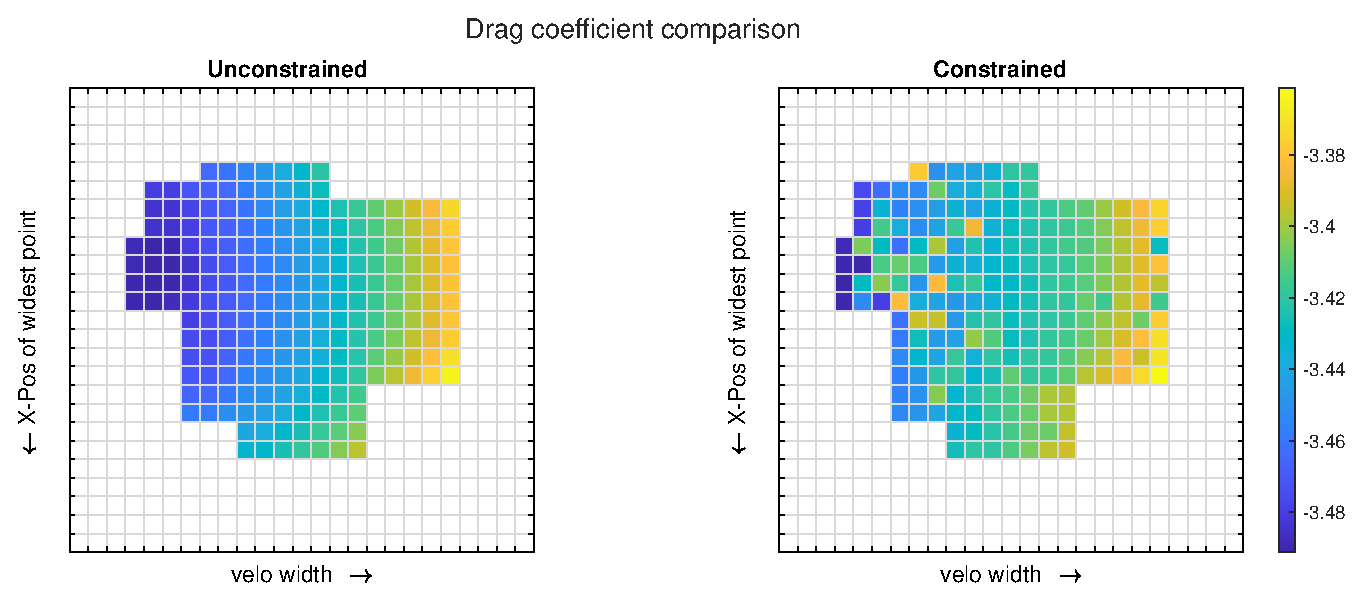
\includegraphics[width=1\linewidth]{bilder/2pt500Samples/dragMapComparison}
	\caption{Karte der Luftwiderstandswerte der Lösungen}
	\label{fig:1stmapDrag}
\end{figure}

In Abb. \cref{fig:1stmapDrag} sind die Karten von Luftwiderstandskoeffizienten der produzierten Ergebnisse in beiden Versionen aufgeführt.
Die Karte ohne Constraint bestätigt die Hypothese, dass breitere Velomobile mit schlechterem Luftwiderstandskoeffizienten korreliert sind.
Auch ist erkennbar, dass es ein mittleres Optimum bezüglich der x-Position dieses Punktes zu geben scheint, da Luftwiderstandswerte sowohl bei Abweichungen nach oben als auch bei Abweichungen nach unten schlechter werden.
Dass die oben aufgestellte Hypothese bestätigt werden kann und die Karte einen graduellen Verlauf aufweist, sind Zeichen für die korrekte Funktionalität des Algorithmus.
Im Gegensatz dazu ist die Karte der Variante mit Constraint wesentlich unregelmäßiger.
Dies bedeutet allerdings nicht, dass der Algorithmus in dieser Variante nicht korrekt arbeitet, die Unregelmäßigkeit der Karte rührt daher, dass die Fitness des Algorithmus aus einer Kombination von Luftwiderstandskoeffizienten und Constraint zusammensetzt.
Auch bewegen sich die Luftwiderstandswerte, wie bereits anhand der Boxplots sichtbar war im Bereich.
Besonders gute Lösungen bezüglich einer dieser beiden Komponenten können fehlende Optimalität bezüglich der anderen damit ausgleichen.
Trotzdem sind auch in dieser Karte die gleichen zugrundeliegenden Tendenzen zu erkennen.
Breitere Velomobile sind auch hier schlechter bezüglich des Luftwiderstands und Optimalität sinkt nach unten und oben.
Interessant ist, dass am rechten, sprich breiteren, Ende einige Lösungen gefunden wurden die sogar bessere Luftwiderstandswerte aufweisen als deren Gegenstücke in der Variante ohne Constraint.
Und auch wenn auf der linken Seite einige Lösungen existieren, welche erheblich schlechtere Luftwiderstandswerte aufweisen wie ihre Gegenstücke, so existieren auch sehr viele mit vergleichbaren Werten.
Um solche Verschlechterungen in Kontext setzten zu können müssen sich die Karten des Constraints angeschaut werden.

\begin{figure}[h]
	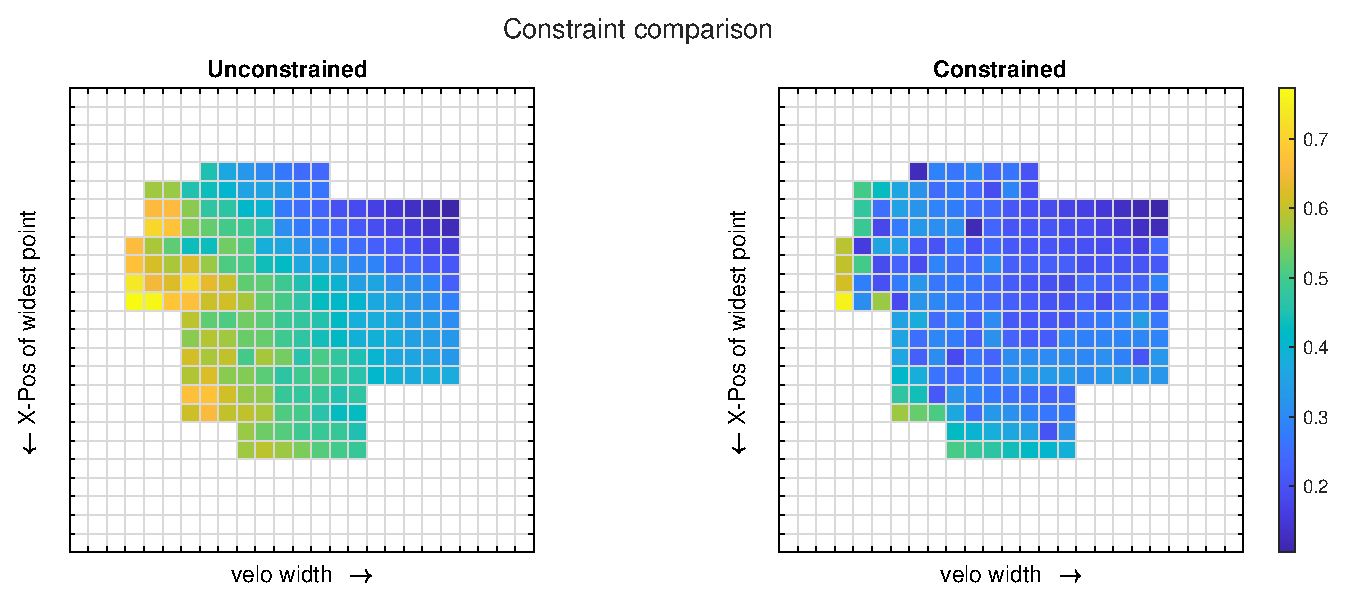
\includegraphics[width=1\linewidth]{bilder/2pt500Samples/constraintMapComparison}
	\caption{Karte der Constraintwerte der Lösungen}
	\label{fig:1stmapCon}
\end{figure}

In Abb. \cref{fig:1stmapDrag} sind die Karten der korrespondierenden Constraint-Werte für beide Varianten zu sehen.
Ersteinmal lässt sich auch hier die Hypothese bestätigen, dass breitere Velomobile den Constraint besser erfüllen.
Interessant ist allerdings auch, dass ohne Einbindung des Constraints, Lösungen, deren breitester Punkt weiter vorne ist den Constraint besser erfüllen.

Im Vergleich der beiden Karten ist noch viel stärker, als den Boxplots, ersichtlich welchen Effekt die Einbindung des Constraints hat.
Es ist klar ersichtlich wie viel besser ein Großteil der Lösungen den Constraint erfüllen.
Besonders stark is dieser Effekt im Mittelfeld der Karte in denen sich Constraintwerte halbieren und teilweise noch stärker verringern.
Zum rechten extremen Rand schwächt die Constraintverbesserung ab, da dortige Radkästen so breit sind, dass selbst die Variante ohne Constraint diesen leicht erfüllen kann.
Auch ist hervorzuheben, dass sich Verbesserungen bis zum linken Rand der Individuen durchziehen.
Selbst in der linken, sprich schmalsten Spalte, ist eine Verbesserung der Individuen erkennbar, und die nächste Spalte enthält bereits ein Individuum welches nahe der besten gefundenen Constraint-Werte angesiedelt ist.

\begin{figure}[h]
	\centering
	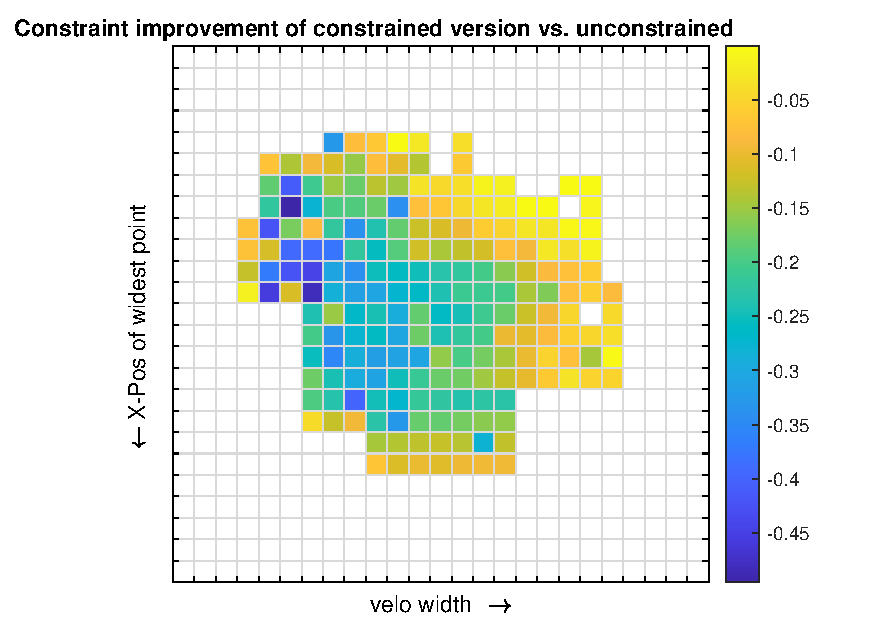
\includegraphics[width=.7\linewidth]{bilder/2pt500Samples/constraintImprovements}
	\caption{Verbesserungen des Constraints zwischen Version ohne und mit Constraint}
	\label{fig:1stmapConCompare}
\end{figure}

In Abb. \cref{fig:1stmapConCompare} ist die Verbesserung der Constraintwerte von der Version ohne Constraint zur Version mit Constraint dargestellt.
Der bereits oben erwähnte Effekt, dass die größten Verbesserungen besonders in der linken Hälfte der Karte stattfinden ist hier noch klarer ersichtlich.
Gerade diese Hälfte ist allerdings die, die bessere Luftwiderstandswerte aufweist und in der die Erfüllung des Constraints aufgrund der geringeren Breite, die Velomobile in diesen Zellen auszeichnet, wesentlich schwerer fällt.
Zusammenfassend kann man sagen, dass die Einbindung des Constraints mit den im ersten Experiment vorliegenden Einschränkungen merkliche Auswirkungen auf das Ergebnis hat.
Auch ist herauszustellen, dass eine starke Verbesserung des Constraints bei einer schwachen Verschlechterung des Luftwiderstands stattfindet.
%Weiterführenden Experimente sollten ohne die Einschränkungen bezüglich Freiheitsgraden und Länge des Experimentes

\subsubsection{Erhöhung der Freiheitsgrade}
\label{sub:exp2nd}
Mit dem ersten Experiment konnte gezeigt werden, dass der Algorithmus sowohl Luftwiderstandskoeffizienten als auch Constraint optimiert, und dabei relativ geringe Kosten in Bezug zum erreichten Luftwiderstand entstehen.
Das erste Experiment hatte allerdings einige Einschränkungen, bezüglich der Parametrisierung um es einfach zu halten.
Die erste dieser Einschränkungen war die Reduzierung auf Deformation in 2 Punkten, sprich 6 Freiheitsgraden.
Diese Reduzierung half dabei das Problem klein zuhalten, hatte aber eine erhebliche Einschränkung des Lösungsraums zur Folge.
Ziel des zweiten Experiments ist es die Anzahl an Freiheitsgraden erheblich zu erhöhen, damit die Zahl an möglichen Deformationen erheblich zu erhöhen, was den positiven Effekt der Einbindung eines Constraints hoffentlich verstärkt.

\begin{figure}[h]
	\centering
	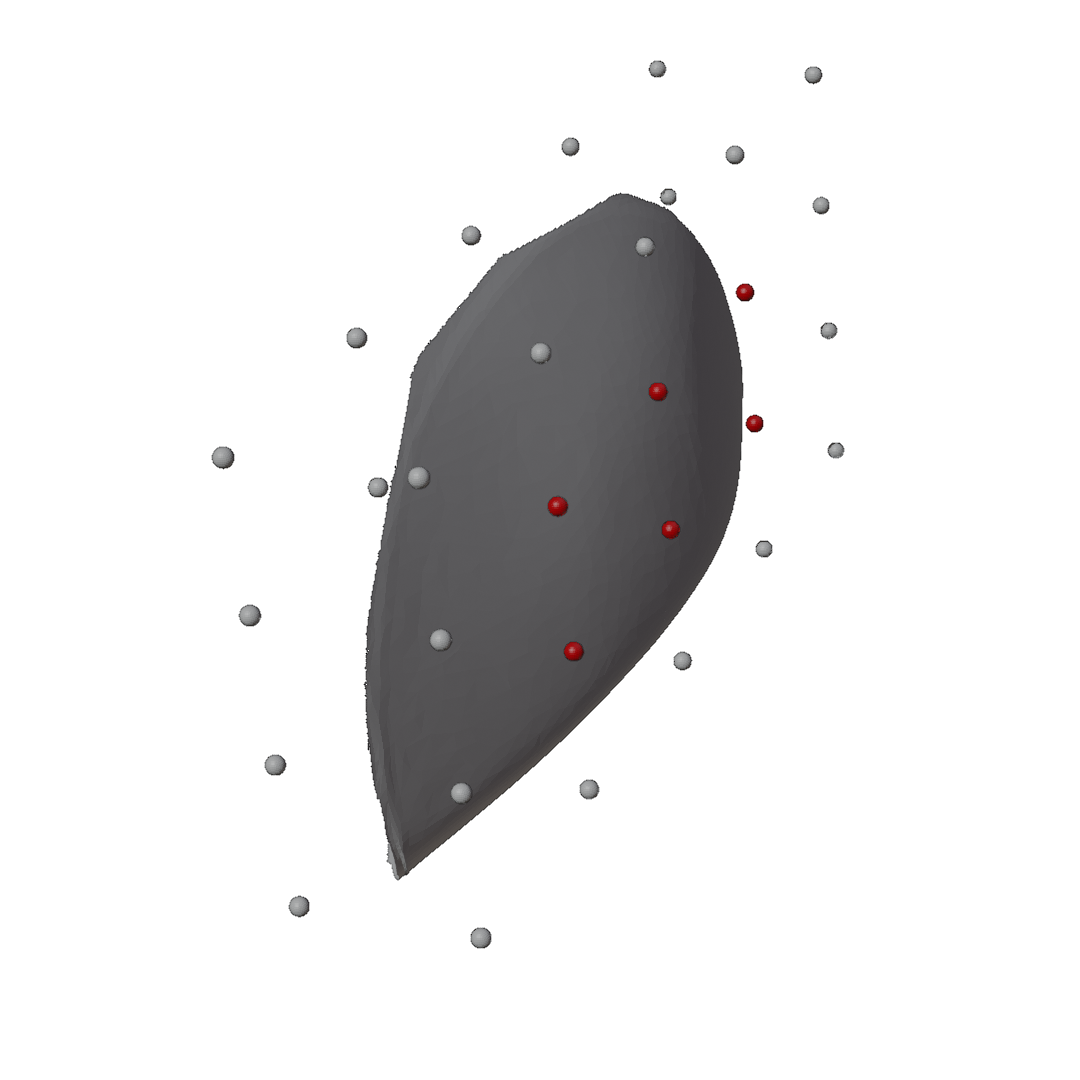
\includegraphics[width=.7\linewidth]{bilder/6ptDeformationPoints}
	\caption{Deformationspunkte des 2. Experiments}
	\label{fig:ffd2nd}
\end{figure}
Die in \cref{fig:ffd2nd} dargestellte Deformationspunkte wurden mit einigen Vorüberlegungen gewählt.
Die Anzahl an horizontaler Reihen wurde von einer auf zwei erhöht um Deformationen , wie ein Auseinanderziehen oder Zusammendrücken in z-Richtung zu erlauben.
Es liegt die Vermutung nahe, dass die im vorigen Experiment gewählten Deformationspunkte die möglichen Phänotypen einschränken, besonders in Anbetracht auf die x-Position des breitesten Punkts.
Da diese eine der Features der MAP-Elites-Karte ist und die Karte im vorigen Experiment entlang dieser Dimension nicht vollständig ausgefüllt wurde, wurde die Anzahl der Deformationspunkte in x-Richtung von 2 auf drei erhöht, um mehr Deformationen zuzulassen, in denen der breiteste Punkt weiter vorne oder hinten liegt.
Insgesamt ergeben sich dadurch 6 Deformationspunkte, welche in alle drei Richtungen bewegt werden können, wodurch sich 18 Freiheitsgrade ergeben.
%Diese Erhöhung ist groß genug

\begin{table}[h]
	\centering
	\begin{tabularx}{.75\textwidth}{ll}\hline
		Anzahl initialer Samples & 100 \\
		Anzahl Samples & 500 \\
		Anzahl neuer Samples pro Akquiseschleife & 20 \\
		Anzahl Generationen Akquise-MAP-Elites & 1024 \\
		Kinder pro Generation Akquise-MAP-Elites & 32 \\
		Anzahl Generationen Ergebnis-MAP-Elites & 2048 \\
		Kinder pro Generation Akquise-MAP-Elites & 32 \\
		Auflösung der MAP-Elites Karte & 25 * 25  \\
		\hline
		%\rowcolor{lightgray}
		Freiheitsgrade & 18 \\
		Mittelwertgewichtung & 1 \\
		Varianzgewichtung & 2 \\
		Constraintgewichtung & 1 \\
	\end{tabularx}
	\label{tab:param2nd}
	\caption{Parametrisierung des zweiten Experiments (Änderungen zum ersten Experiment hervorgehoben)}
\end{table}


\begin{figure}[h]
	\centering
	\begin{minipage}{0.45\textwidth}
		\centering
		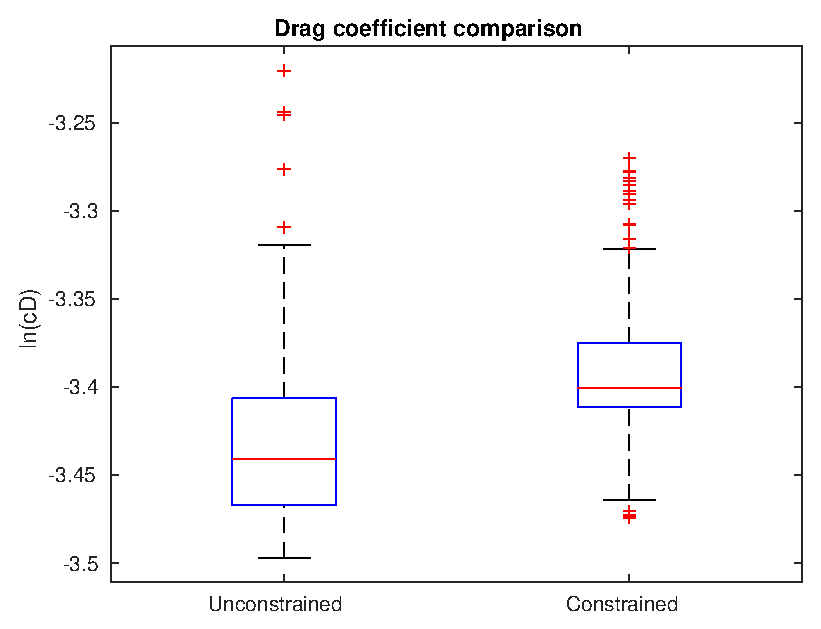
\includegraphics[width=1\linewidth]{bilder/6pt500Samples/dragBoxplot}
		\caption{Vergleich der Luftwiderstände der produzierten Lösungen}
		\label{fig:2nddragbox}
	\end{minipage}\hfill
	\begin{minipage}{0.45\textwidth}
		\centering
		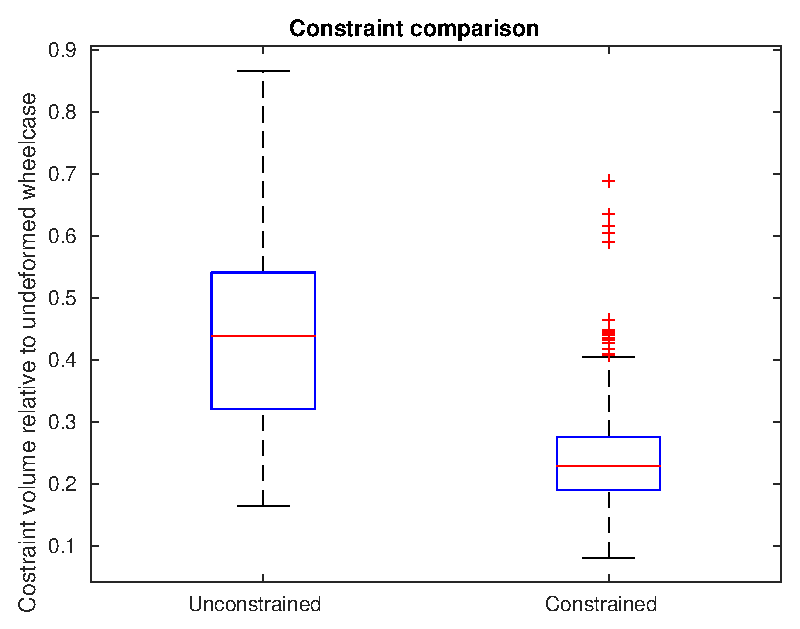
\includegraphics[width=1\linewidth]{bilder/6pt500Samples/constraintBoxplot}
		\caption{Vergleich der Constrainterfüllung der produzierten Lösungen}
		\label{fig:2ndconbox}
	\end{minipage}
\end{figure}

Der erste Unterschied, der im Vergleich zum ersten Experiment auftritt, sind die stärkeren Unterschiede in Constraint und Luftwiderstand für.


\begin{figure}[h]
	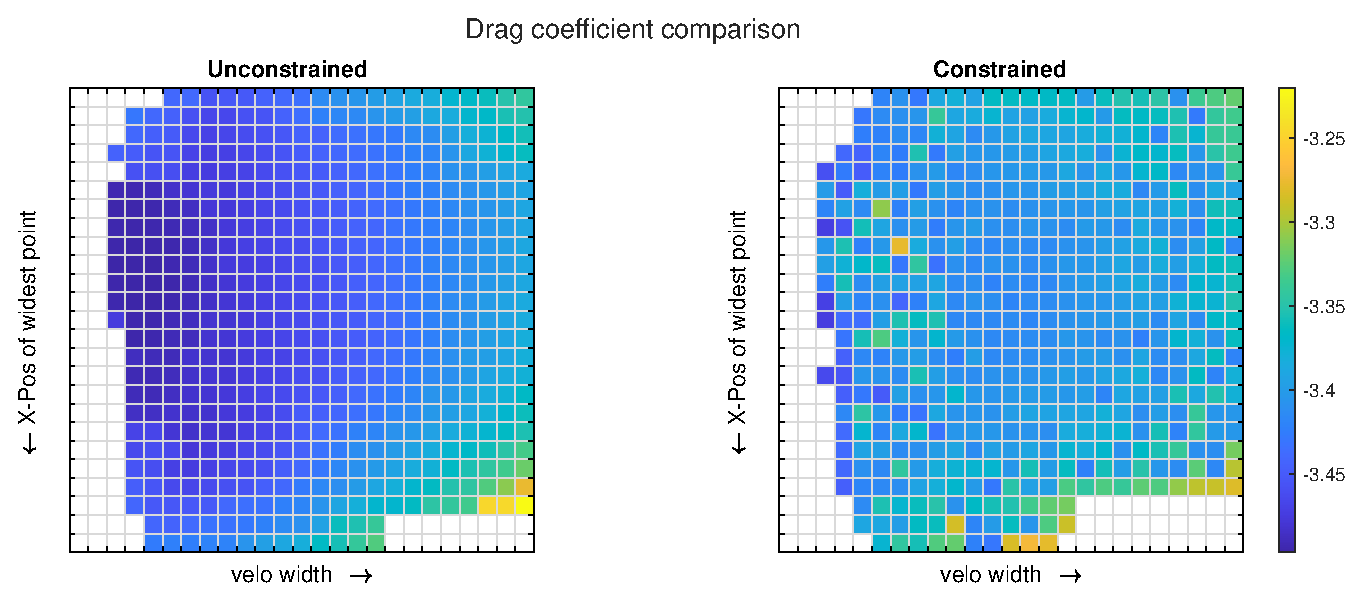
\includegraphics[width=1\linewidth]{bilder/6pt500Samples/dragMapComparison}
	\caption{Karte der Luftwiderstandswerte der Lösungen}
	\label{fig:2ndmapDrag}
\end{figure}

In Abbildungen \cref{fig:2ndmapCon} \cref{fig:2ndmapDrag} ist klar zu Erkennen, dass die Karte aus Lösungen weitaus besser gefüllt wird als beim ersten Experiment.
Die bessere Füllung entlang der Vertikalen ist leicht zu erklären.
Die Aufteilung in 6 Deformationspunkte führt dazu, dass die beiden vorderen weiter vorne liegen, als der vordere aus dem vorigen Experiment und die beiden hinteren entsprechend auch weiter hinten liegen.
Deformationen mit diesen Deformationspunkten können also mehr Lösungen generieren, in denen der breiteste Punkt sehr weit vorne oder sehr weit hinten liegt.
Interessant ist allerdings, dass die Karte auch entlang der Horizontalen  besser gefüllt wird.
An der Stärke der Deformationen in y-Richtung wurde allerdings nichts geändert, es sollte also nicht möglich sein wesentlich breitere Velomobile zu generieren.
\todo{Erklärung warum mehr horiz}

\begin{figure}[h]
	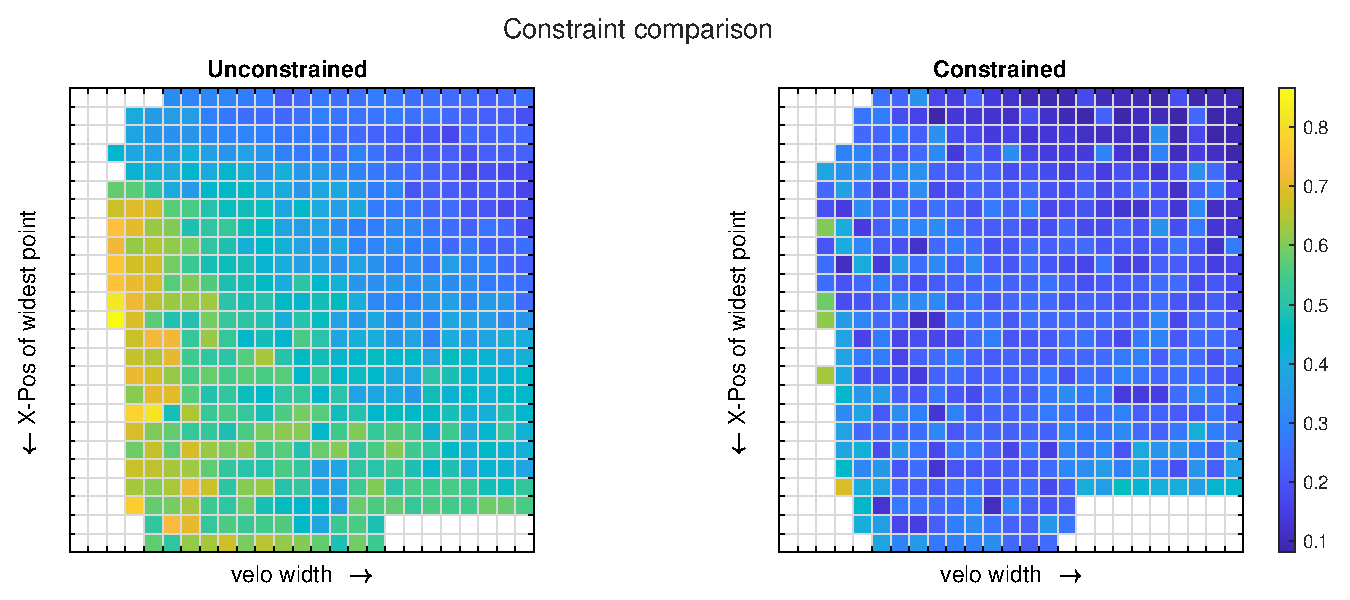
\includegraphics[width=1\linewidth]{bilder/6pt500Samples/constraintMapComparison}
	\caption{Karte der Constraintwerte der Lösungen}
	\label{fig:2ndmapCon}
\end{figure}

Die Karte der Constraints bestätigt auch hier, die im ersten Experiment bereits beobachtete Tendenz, dass der Constraint in breiteren Velomobilen und in solchen in denen der breiteste Punkt weiter vorne liegt einfacher zu erfüllen ist.
Es ist allerdings herauszustellen, dass in der Variante ohne Constraint selbst die Lösungen in der oberen rechten Ecke eine weniger gute Constrainterfüllung aufweisen als die besten Lösungen in der Variante ohne Constraint des ersten Experiments, trotz der Tatsache, dass diese sowohl breiter sind und die breiteste Stelle weiter vorne liegt.
Zwar ist dieser Effekt auch im Vergleich der Varianten ohne Constraint festzustellen, er fällt dort aber wesentlich schwächer aus.
Dies deckt sich mit der Tatsache, dass eine Erhöhung der Freiheitsgrade und die damit verbundene Vergrößerung des Suchraumes schwerer macht ähnlich gute Lösungen bei gleicher Laufzeit zu finden.
Dass der Effekt in der Variante ohne Constraint aber stärker ist bestätigt, dass die Schwierigkeit des zufälligen Erfüllens des Constraints ohne spezielle Behandlung stärker wächst, als die Schwierigkeit der Erfüllung unter Beachtung des Constraints.

\begin{figure}[h]
	\centering
	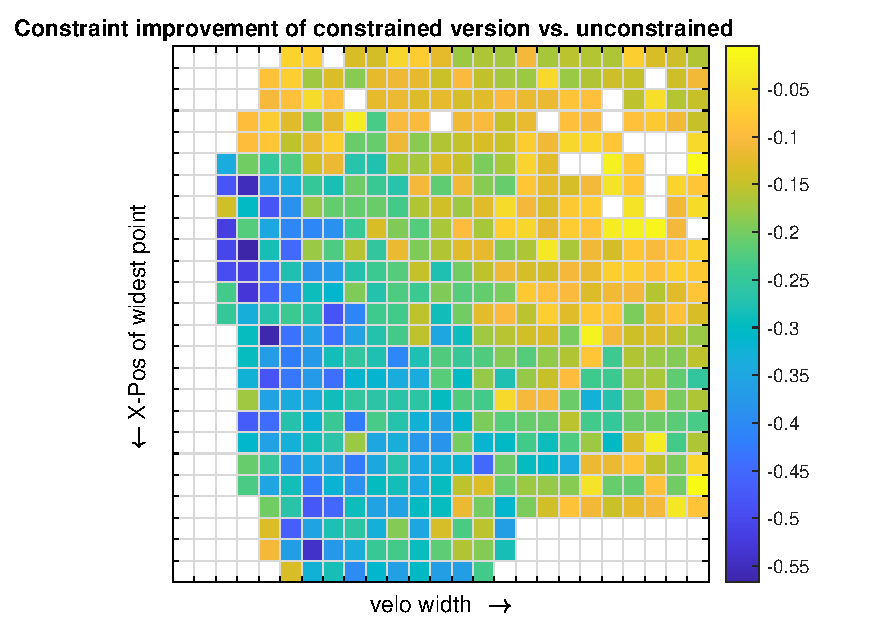
\includegraphics[width=.7\linewidth]{bilder/6pt500Samples/constraintImprovements}
	\caption{Verbesserungen des Constraints zwischen Version ohne und mit Constraint}
	\label{fig:2ndmapConCompare}
\end{figure}

Es fällt ein interessanter Unterschied zum ersten Experiment auf.
Die Karten der Variante ohne Constraint und der mit Constraint sind im Gegensatz diesen nicht mehr gleich.
Stattdessen ist die Karte ohne Constraint besser gefüllt als die mit Constraint.
Dies fällt vor allem an den Rändern der Karten auf.
Das kann damit zusammenhängen, dass durch die Einführung des Constraints Exploration in Bereichen in denen der Constraint verletzt ist weniger stattfindet.
Außerdem besteht die Vermutung, dass weite Teile des Problemraums den Constraint nicht erfüllen, sondern stark verletzen.

%\missingfigure{boxplots akquiseindividuen}

Zur definitiven Auswertung sollte allerdings sichergestellt sein, dass Akquise- und Ergebnis-MAP-Elites ausreichend konvergiert sind.
Dass kann aus in diesem Experiment noch nicht definitiv festgestellt werden.
Um eine definitive Aussage über Konvergenz treffen zu können sollte das Experiment unter ausführlicheren Bedingungen wiederholt werden.

\subsubsection{Erhöhung der Laufzeit}
\label{sub:exp3rd}
\begin{table}[h]
	\centering
	\begin{tabularx}{.75\textwidth}{ll}\hline
		Anzahl initialer Samples & 100 \\
		%\rowcolor{lightgray}
		Anzahl Samples & 1000 \\
		Anzahl neuer Samples pro Akquiseschleife & 20 \\
		%\rowcolor{lightgray}
		Anzahl Generationen Akquise-MAP-Elites & 2048 \\
		Kinder pro Generation Akquise-MAP-Elites & 32 \\
		%\rowcolor{lightgray}
		Anzahl Generationen Ergebnis-MAP-Elites & 8192 \\
		Kinder pro Generation Akquise-MAP-Elites & 32 \\
		Auflösung der MAP-Elites Karte & 25 * 25  \\
		\hline
		Freiheitsgrade & 18 \\
		Mittelwertgewichtung & 1 \\
		Varianzgewichtung & 2 \\
		Constraintgewichtung & 1 \\
	\end{tabularx}
	\label{tab:params3rd}
	\caption{Parametrisierung des dritten Experiments (Änderungen zum zweiten Experiment hervorgehoben)}
\end{table}

Die zweite Einschränkung der beiden vorigen Experimente war die Beschränkung auf eine kleinere Anzahl an ausgewerteten Samples und Generationen in Akquise- und Ergebnis-MAP-Elites.
Durch die Beschränkung auf eine kleinere Anzahl an Samples besteht die Möglichkeit, dass der Suchraum nicht präzise genug und/oder nicht weitläufig genug abgebildet wurde.
Die Beschränkung in Generationen des Akquise- und Ergebnis-MAP-Elites kann dazu führen, dass diese noch nicht vollständig konvergiert sind.
Da die Überlegung nahe liegt, dass die Variante mit Constraint länger benötigen könnte um ausreichend zu konvergieren, sollte untersucht werden ob die Erhöhung dieser Parameter zu signifikanten Änderung im Vergleich zur kürzeren Version führt, indem die Gewinne nach 500 Samples und 1024 bzw. 2048 Generationen quantifiziert werden.

Auf ersten Blick sehen die Ergebnisse des dritten Experiments denen des zweiten Experiments sehr ähnlich.
Die Karten werden etwas besser gefüllt, was durch Erhöhung der Zahl der ausgewerteten Samples und der Akquise- und Ergebnisgenerationen grundsätzlich zu erwarten war.

\begin{figure}[h]
	\centering
	\begin{minipage}{0.45\textwidth}
		\centering
		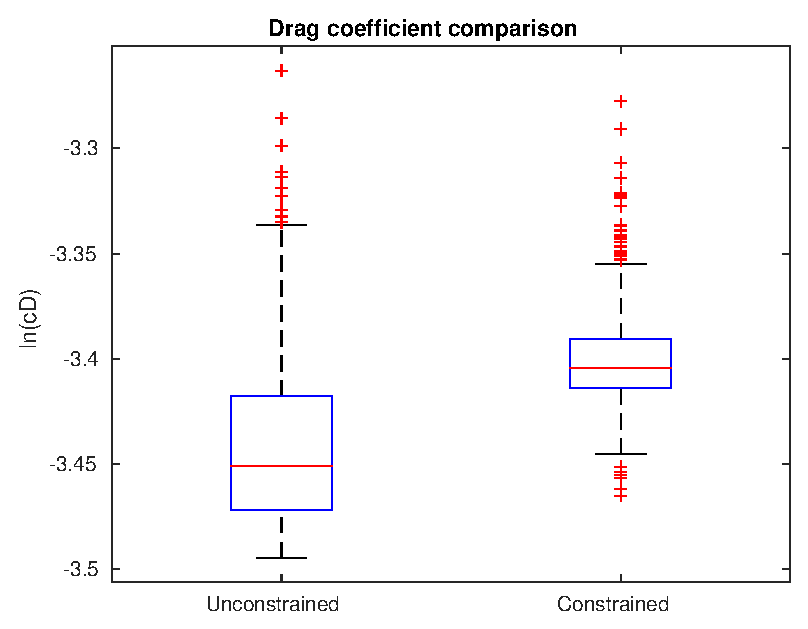
\includegraphics[width=1\linewidth]{bilder/6pt1000Samples/dragBoxplot}
		\caption{Vergleich der Luftwiderstände der produzierten Lösungen}
		\label{fig:3rddragbox}
	\end{minipage}\hfill
	\begin{minipage}{0.45\textwidth}
		\centering
		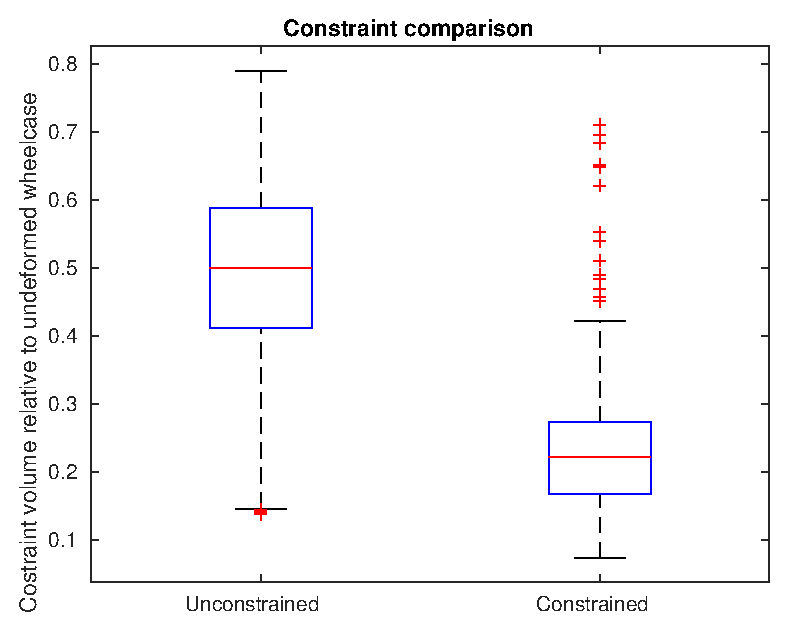
\includegraphics[width=1\linewidth]{bilder/6pt1000Samples/constraintBoxplot}
		\caption{Vergleich der Constrainterfüllung der produzierten Lösungen}
		\label{fig:3rdconbox}
	\end{minipage}
\end{figure}

Die Luftwiderstandskoeffizienten der Variante ohne Constraint haben sich nicht verändert, während bei der Variante mit Constraint ist eine leichte Verbesserung zu verzeichnen.
Dies deckt sich mit der Vermutung, dass die Variante mit Constraint mehr Zeit benötigt um ausreichend auszukonvergieren.
Interessant ist auch die Veränderung der Constraintwerte.
Hier ist bei der Variante mit Constraint keine nennenswerte Änderung zu verzeichnen, die Constraintwerte der Variante ohne Constraint verschlechtern sich allerdings.
Das ist durchaus interessant, da es bedeuten kann, dass die weitere feine Optimierung bezüglich des Luftwiderstands im Laufe des Algorithmus eine Abkehr von solchen Lösungen darstellt, die den Constraint besser erfüllen.
Das dieser Trend in der Variante ohne Constraint nicht zu beobachten ist ein großer Vorteil.
Auch ist das interessant, da kein nennenswerter Gewinn bezüglich des Luftwiderstands zwischen ersten und zweitem Experiment zu beobachten ist.

\begin{figure}[h]
	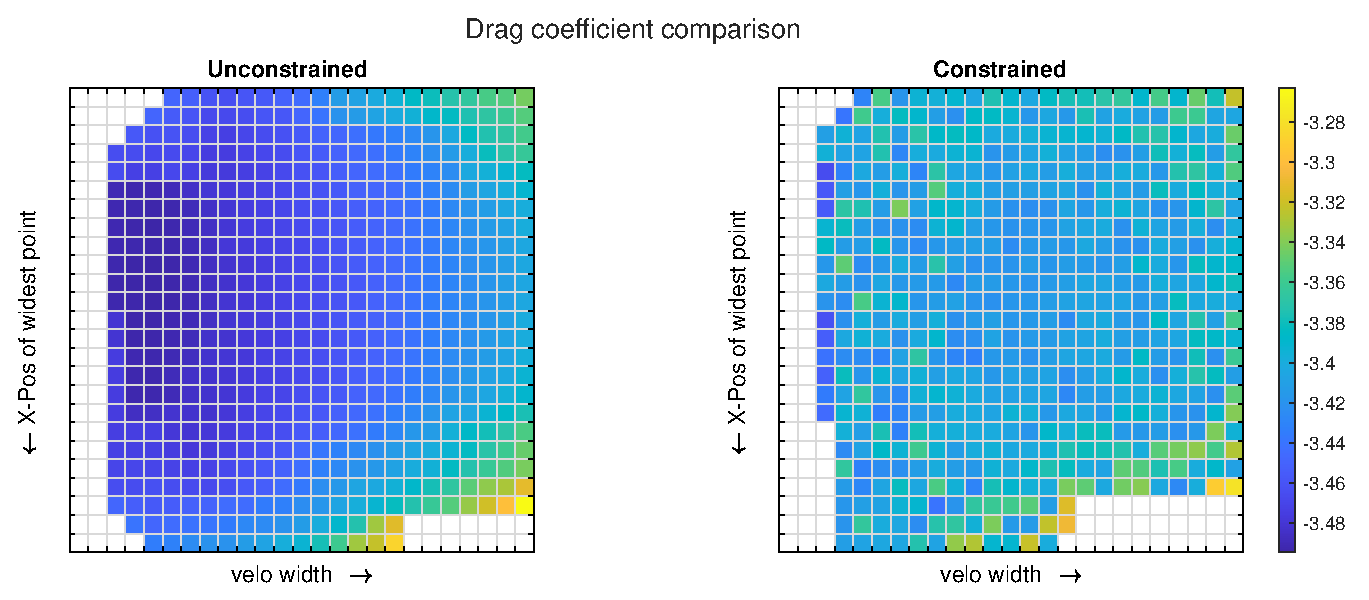
\includegraphics[width=1\linewidth]{bilder/6pt1000Samples/dragMapComparison}
	\caption{Karte der Luftwiderstandswerte der Lösungen}
	\label{fig:3rdmapDrag}
\end{figure}

In \cref{fig:3rdmapDrag} ist der Vergleich der Luftwiderstände der berechneten Lösungen der beiden Versionen dargestellt.
Die Karte der Variante ohne Constraint bestätigt noch einmal die in \cref{sub:exp1st,sub:exp2nd} bereits beobachteten Trends, dass die Breite des Velomobils negativ mit dem Luftwiderstandskoeffizienten korreliert ist und ein mittiges Optimum bezüglich der x-Koordinate des breitesten Punkts existiert.
Es ist festzustellen, dass die Karte etwas besser gefüllt wird als dies noch beim zweiten Experiment der Fall war, dieser Unterschied ist allerdings nur minimal.
Außerdem kann an dieser Karte besser als an den vorigen Karten gesehen werden, dass eine Minimalbreite des Velomobils existiert.
Auch wenn Deformationen nach innen erlaubt werden können diese keinen Einzug in die Karte halten, da alle Lösungen, bei denen sich der breiteste Punkt am Rand des Radkastens befindet, in die gleiche Spalte eingeordnet werden.

\begin{figure}[h]
	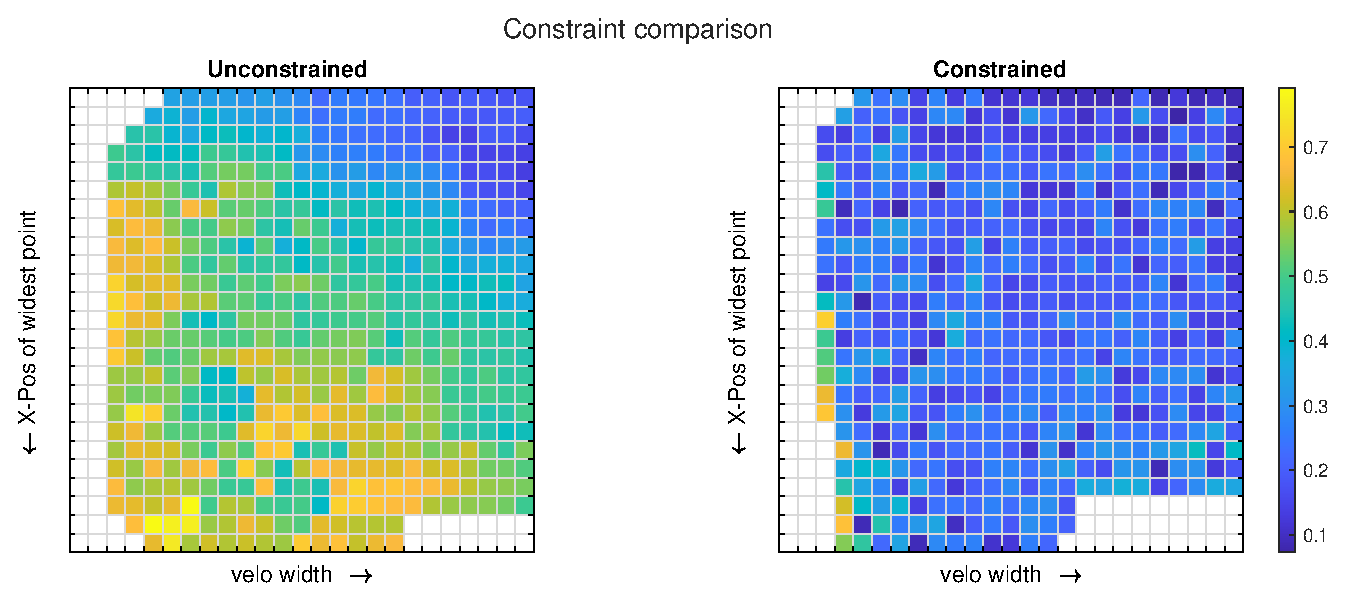
\includegraphics[width=1\linewidth]{bilder/6pt1000Samples/constraintMapComparison}
	\caption{Karte der Constraintwerte der Lösungen}
	\label{fig:3rdmapCon}
\end{figure}

Auch der Vergleich der Constraintwerte der finalen Lösungen beider Varianten,  der in \cref{fig:3rdmapCon} abgebildet ist, bestätigen sich bereits vorher festgestellte Tendenzen.
Die interessanteste Änderung zum zweiten Experiment stellt dabei eine Verschlechterung der Constraintwerte der Variante ohne Constraint im linken unteren Dreieck der Karte dar.
Hier bestätigt sich die bei der Betrachtung der Boxplots gemachte Beobachtung, dass vom zweiten aufs dritte Experiment eine Verschlechterung der Constraintwerte stattfindet.
An der Karte ist zusätzlich noch zu erkennen, dass dies keine globale Verschlechterung ist, sondern diese nur bestimmte Regionen der Karte betrifft.
Dies ist besonders wichtig, da der linke Bereich der Karte, der Bereich ist in dem die Luftwiderstandswerte am besten sind, und damit genau der Bereich ist in dem die Lösungen attraktiver sind.
Dass eine Erhöhung der Generationen für Akquise und Ergebnis-MAP-Elites die Verschlechterung von Lösungen bezüglich des Constraints zur Folge hat, wenn dieser nicht explizit behandelt wird, deutet darauf hin, dass die Variante mit Constraint bei längeren Laufzeiten im Vergleich zur Variante ohne Constraint besser abschneidet. 

\begin{figure}[h]
	\centering
	\begin{minipage}{0.45\textwidth}
		\centering
		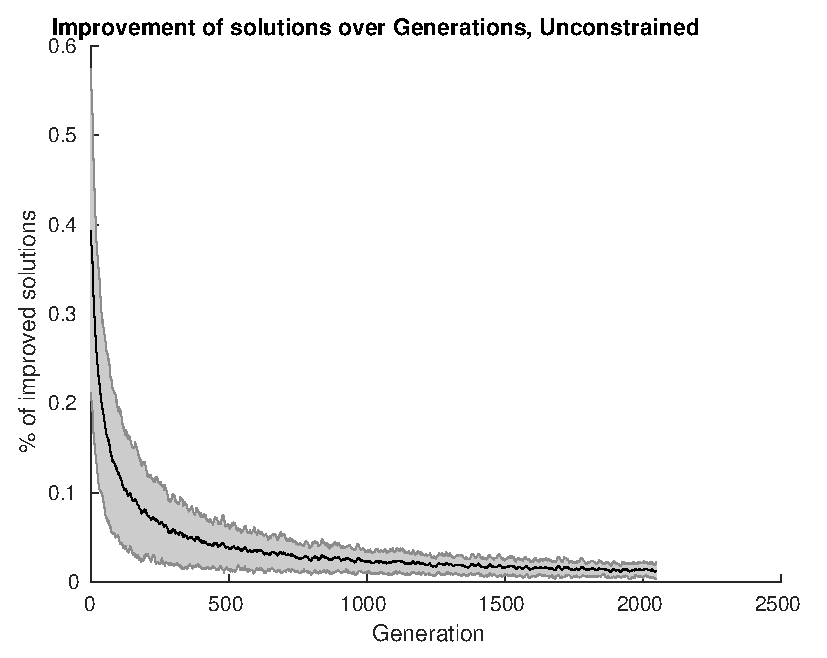
\includegraphics[width=1\linewidth]{bilder/6pt1000Samples/acqImprovementsUncon}
		\caption{Prozentuale Verbesserung der Samples in Akquisegenerationen in Version ohne Constraint}
		\label{fig:acqImprovementUncon}
	\end{minipage}\hfill
	\begin{minipage}{0.45\textwidth}
		\centering
		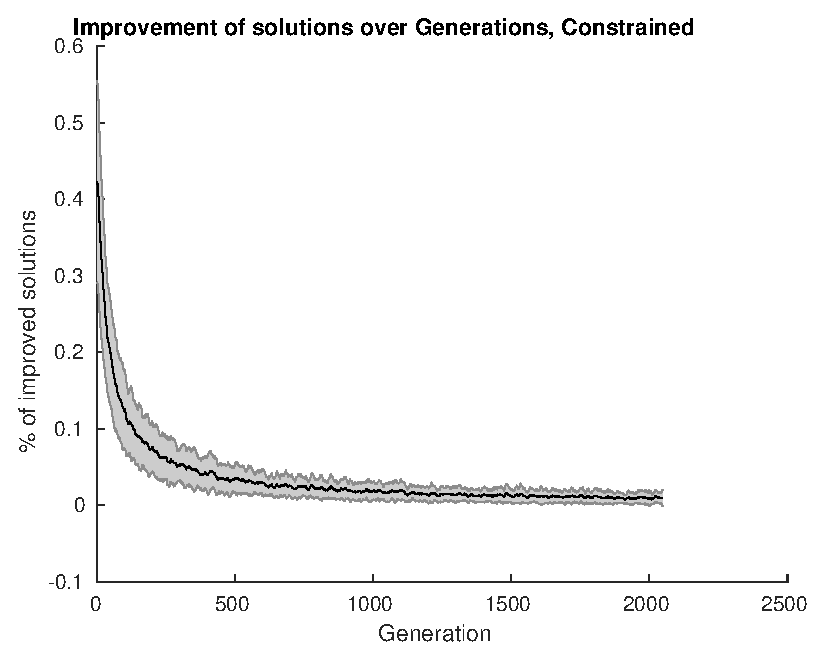
\includegraphics[width=1\linewidth]{bilder/6pt1000Samples/acqImprovementsCon}
		\caption{Prozentuale Verbesserung der Samples in Akquisegenerationen in Version mit Constraint}
		\label{fig:acqImprovementCon}
	\end{minipage}
%	\todo{merge graphs}
\end{figure}

In \cref{fig:acqSamplesUncon,fig:acqImprovementCon} sind die prozentualen Verbesserungen von Individuen der Akquise-MAP-Elites dargestellt.
Die prozentualen Verbesserungen aller generierten Akquisekarten wurden gemittelt und mit einem gleitenden Mittelwert geglättet.
Mit dem $2\sigma$ Intervall wurde gleichermaßen verfahren.
Es ist klar erkennbar, dass beide Variante über die Generationen konvergieren.

\begin{figure}[h]
	\centering
	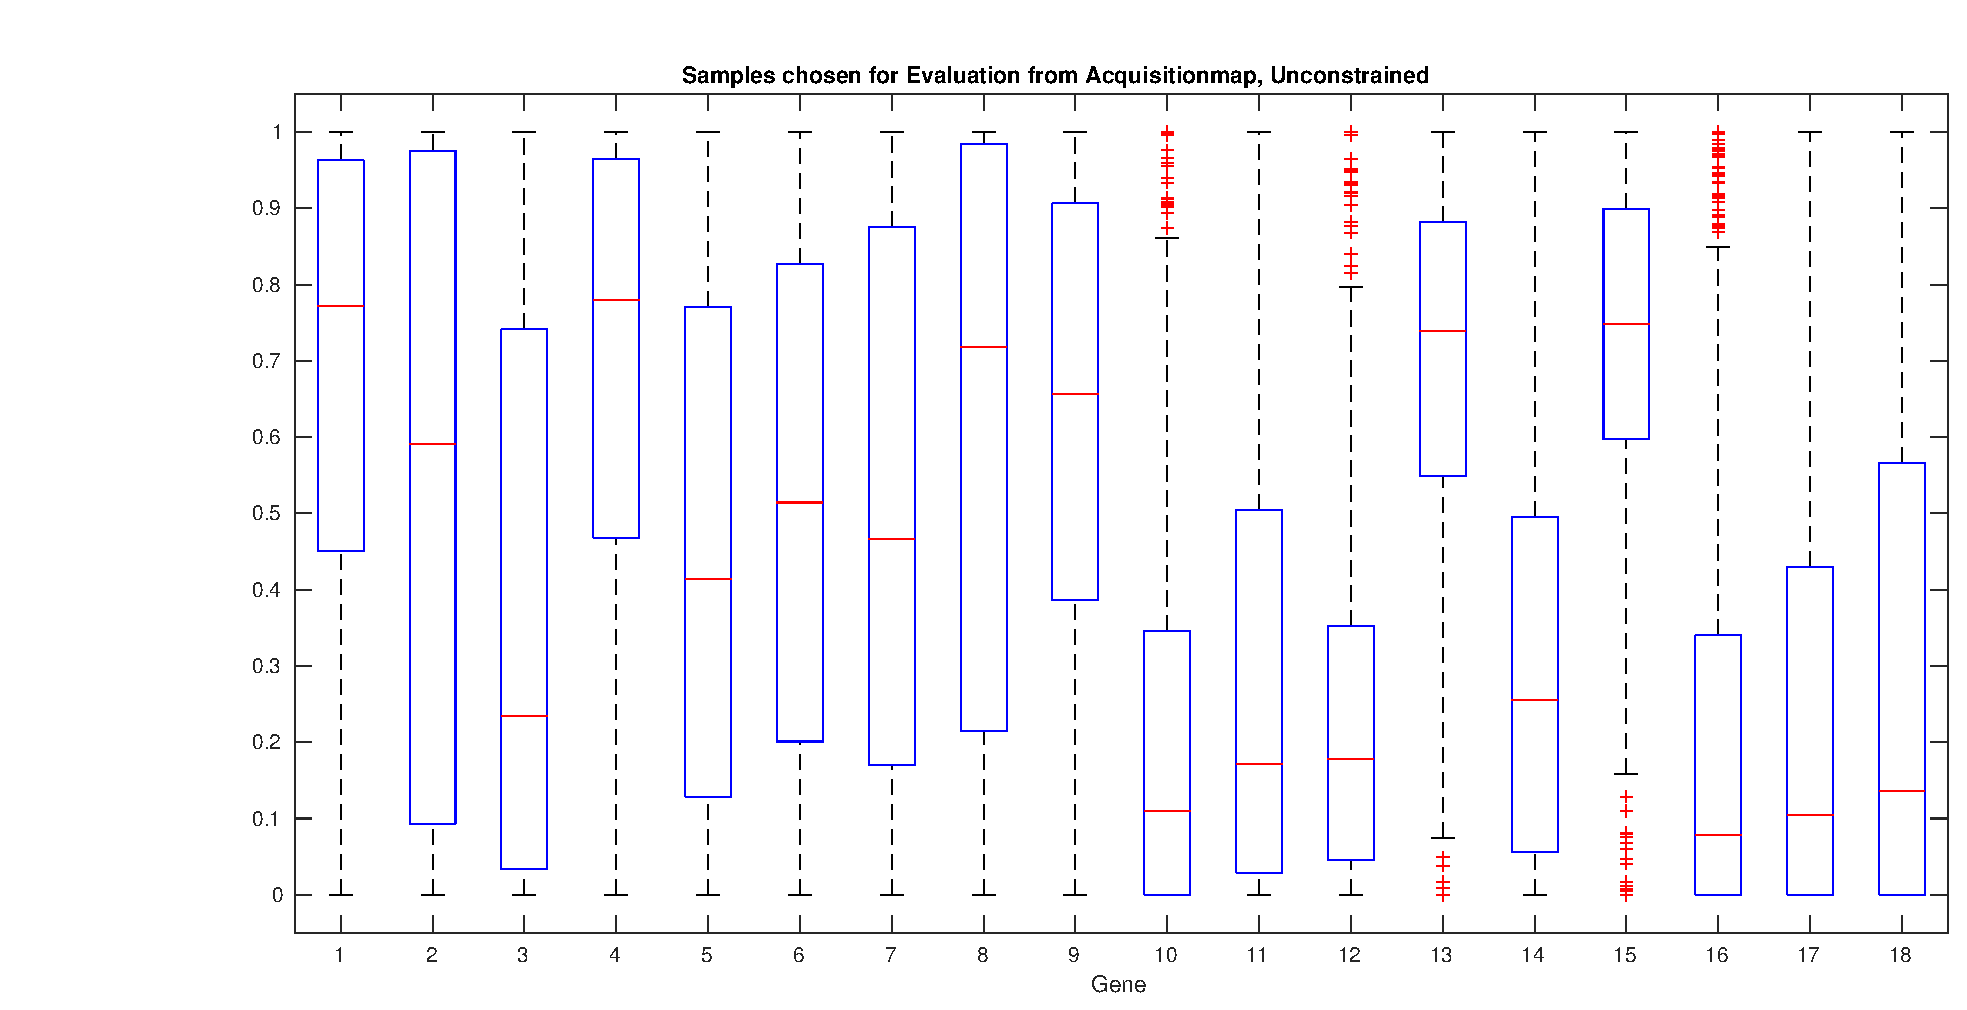
\includegraphics[width=1\linewidth]{bilder/6pt1000Samples/acquisitionDiversityUncon}
	\caption{Genotypen, der für präzise Evaluation ausgewählten Individuen (ohne Constraint)}
	\label{fig:geneticDivUncon}
\end{figure}

\Cref{fig:geneticDivCon,fig:geneticDivUncon} zeigen die Genotypen der zur präzisen Auswertung ausgewählten Individuen in beiden Varianten.
Jeder Boxplot repräsentiert dabei ein Gen des Genotyps.
Da in dieser Variante mit 18 Freiheitsgraden gearbeitet wurde ergeben sich 18 Gene.
Alle Werte sind auf das Intervall $[0;1]$ skaliert wobei 0 die minimale (negative) Deformation und 1 die maximale Deformation darstellt.
Zuerst ist festzustellen, dass der genetische Raum in beiden Varianten gut ausgefüllt wird.
Der Großteil der Gene deckt das gesamte Intervall $[0;1]$ in deren $2\sigma$ Intervall ab.
In beiden Varianten existieren fünf unterschiedliche Gene, die das nicht tun, alle dieser Gene weisen allerdings Ausreißer über das gesamte Intervall aus und mit Ausnahme der Gene 13-15 der Variante mit Constraint decken sie das Intervall mit ihrem $2\sigma$ Intervall beinahe ab.
Die Tatsache, dass der genetische Problemraum vollständig ausgefüllt wird, ist ein Zeichen, dass nicht zu viele Freiheitsgrade oder zu wenige präzise Funktionsauswertungen genutzt wurden.
Das Mapping von Genotyp auf FFD-Deformation fand nach dem folgenden Schema statt:
\begin{enumerate}
	\item[1-3] x-Deformation der drei unteren Deformationspunkte
	\item[4-6] x-Deformation der drei oberen Deformationspunkte
	\item[7-9] y-Deformation der drei unteren Deformationspunkte
	\item[10-12] y-Deformation der drei oberen Deformationspunkte
	\item[13-15] z-Deformation der drei unteren Deformationspunkte
	\item[16-18] z-Deformation der drei oberen Deformationspunkte
\end{enumerate}

Einige dieser Tripletts sind entweder in sich selbst interessant andere weisen interessante Unterschiede zwischen den beiden Varianten auf.

Das erste besondere Triplett sind die Gene 10-12.
Diese sind für die Deformation in y-Richtung der oberen Reihe der Deformationspunkte verantwortlich.
In der Variante ohne Constraint fällt auf, dass das gesamte Triplett sehr stark zu kleinen Werten tendiert. 
Bei allen drei Genen liegt das obere Quartil unter $0,5$ und der Median um $0,2$.
Dies ist eine starke Tendenz zu schwachen beziehungsweise teilweise negativen Deformationen in y-Richtung.
Das in der Auswahl der Akquiseindividuen so eine starke Tendenz bezüglich einer der Richtungen existiert lässt darauf schließen, dass in Bereichen mit niedrigen Deformationen der oberen Punkte in y-Richtung mehr Exploitation stattfindet.
Besonders interessant ist dies vor allem, wenn man die gleichen Gene in der Version mit Constraint betrachtet.
Dort ist die gegensätzliche Tendenz zu erkennen.
Zwar fällt die Tendenz zu $1$ hier weniger stark aus, als die zu $0$ in der Variante ohne Constraint, so ist es doch eine merkliche Tendenz, die durch die Tatsache, dass sie die vorige völlig umkehrt, noch interessanter wird.
Die Einführung des Constraints macht Bereiche, die diesen nicht gut erfüllt unattraktiver zur Exploitation.
Es ist naheliegend, dass die Deformationen in y-Richtung die sind, die den stärksten Einfluss auf die Erfüllung des Constraints haben.
Ebenso ist naheliegend, dass negative Deformationen in y-Richtung den Constraint voraussichtlich nicht gut erfüllen werden.
An der Beobachtung, dass der Trend nicht nur neutralisiert, sondern umgekehrt wird, ist erkennbar wie wichtig diese Deformationen zur Erfüllung des Constraints sind.

Diese Beobachtung ist vor allem im Vergleich zu den anderen drei Genen, die auf eine y-Deformation abgebildet werden (7-9) signifikant.
Bei diesen sind weder so starke Tendenzen, noch eine so starke Umkehr zu beobachten.
Daraus kann geschlussfolgert werden, dass y-Deformationen der oberen Reihe signifikante Teile der Lösung des Problems darstellen.
Besonders unter dem Blick das diese Gene sowohl zur Optimierung des Luftwiderstands, als auch zur Optimierung des Constraints wichtig sind und diese Gene damit ein Spannungsfeld zwischen diesen beiden Zielen darstellt sollte die Signifikanz dieser Gene für das Problem herausgestellt werden.

Das zweite interessante Triplett sind die Gene 13-15.
Diese werden Deformationen der unteren Reihe an Deformationspunkten in z-Richtung abgebildet.
In der Variante ohne Constraint ist der Unterschied zwischen dem den Genen 13,15 und 14 durchaus interessant.
Offensichtlich scheint das Sampling von Individuen in denen die beiden äußeren Punkte nach oben deformiert werden bevorzugt werden.
Gleichzeitig gilt für den mittleren Punkt das Gegenteil, dieser scheint eher nach unten deformiert\footnote{z-Deformationen sind symmetrisch um $0.5$, alles größer $0,5$ ist Deformation nach oben, alles kleiner $0,5$ Deformation nach unten} zu werden.

Diese Werte dieser Gene sind aber besonders in der Variante mit Constraint interessant.
Hier ist ein sehr starker Trend zu negativen Deformationen erkennbar.
Der Median der Werte dieser Gene liegt für all unter $0,2$.
Die Tendenz den mittleren Punkt stärker nach unten zu deformieren bleibt erhalten
Aber zumindest für die Gene 13 \& 15 ist eine Umkehr von positiven Deformationen in der Variante ohne Constraint zu stark negativen Deformationen in der Variante mit Constraint erkennbar.
Die Gene 13 \& 15 scheinen also moderat wichtig zur Optimierung des Luftwiderstands zu sein, gleichzeitig aber auch signifikant zur Optimierung des Constraints zu sein.
Gleiches gilt auch für Gen 14, nur dass hier die gleichen Tendenzen für beide Optimierungen entstehen.
Im Gegensatz zu dem vorigen Triplett und den Genen 13 \& 15 entsteht hier also kein Spannungsfeld.

\begin{figure}[h]
	\centering
	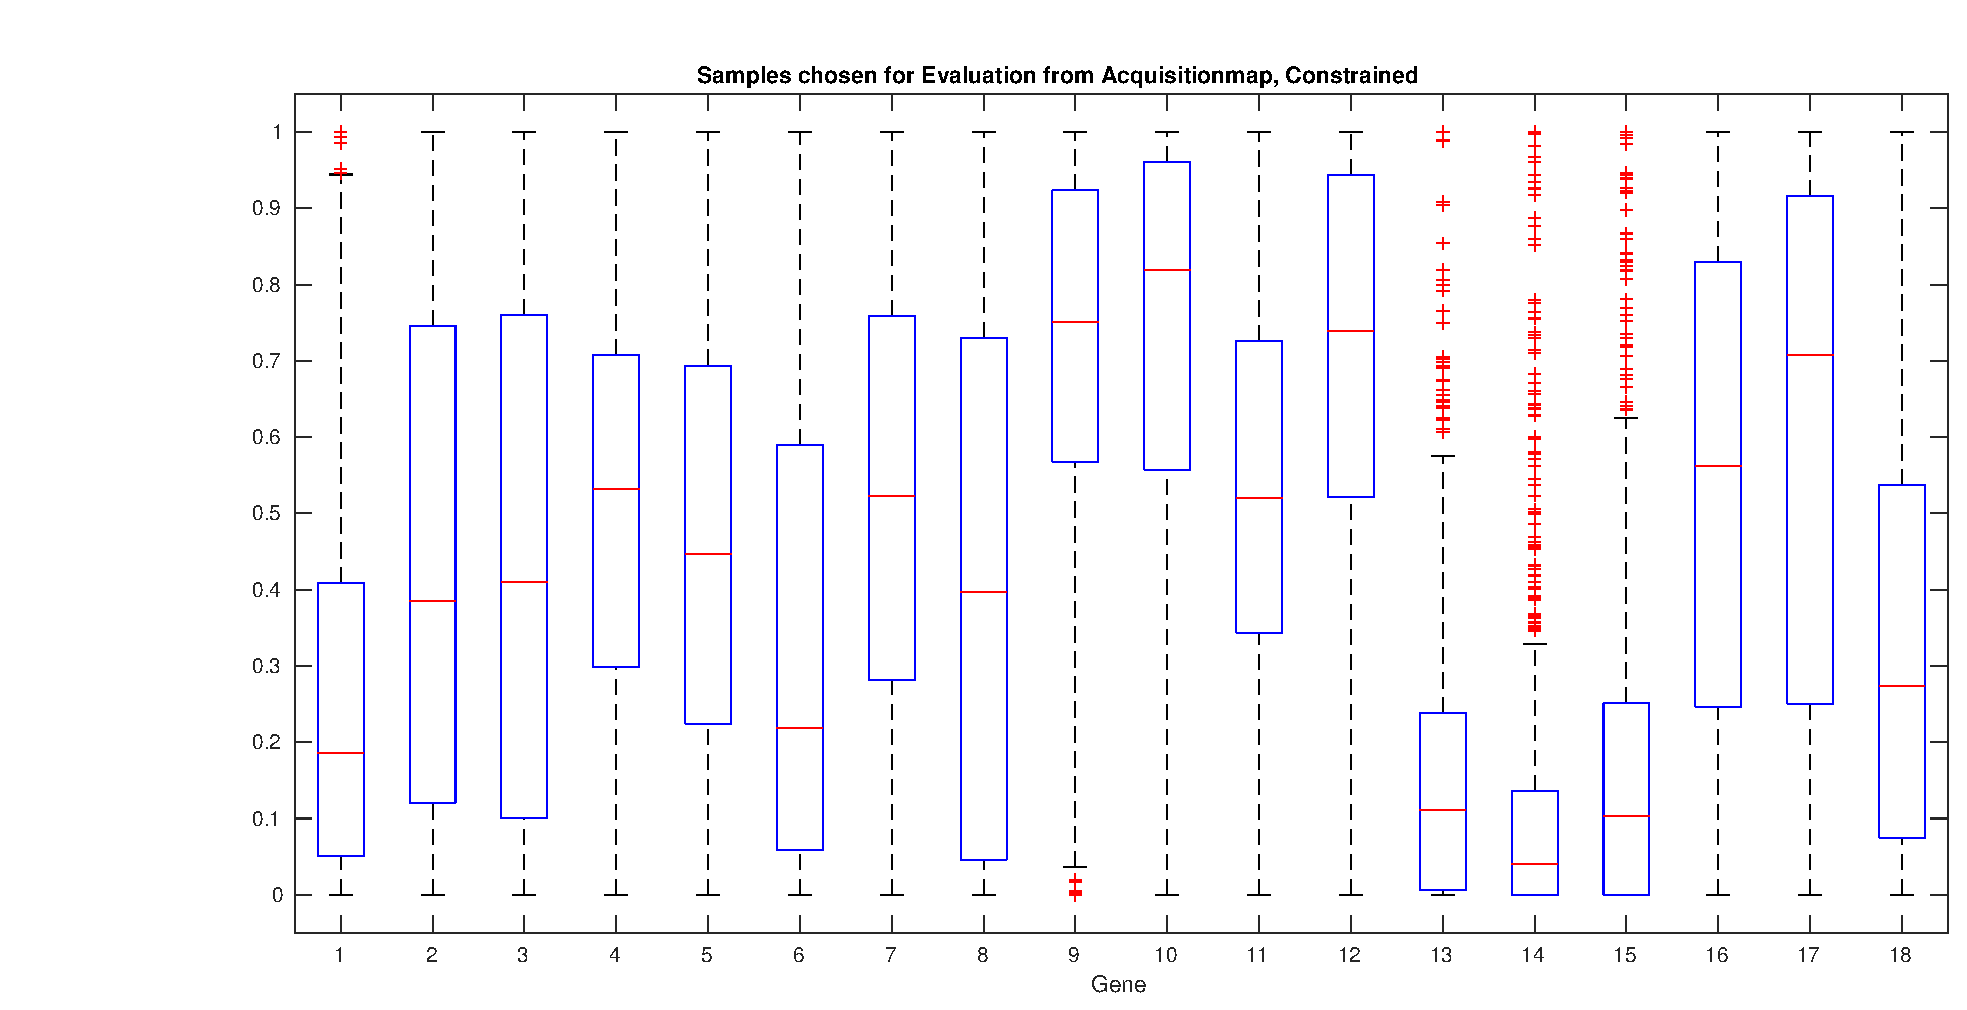
\includegraphics[width=1\linewidth]{bilder/6pt1000Samples/acquisitionDiversityCon}
	\caption{Genotypen, der für präzise Evaluation ausgewählten Individuen (mit Constraint)}
	\label{fig:geneticDivCon}
\end{figure}

Das letzte interessant Triplett sind die Gene 16-18.
Diese werden auf z-Deformationen der oberen Reihe an Deformationspunkten abgebildet.
Hier ist ein Trend zu negativen Deformationen in der Variante ohne Constraint zu erkennen.
Im Vergleich zur Variante ohne Constraint ist für die Gene 16 \& 17 wieder ein umgekehrter Trend zu erkennen, auch wenn dieser nicht so stark wie bei den vorigen beiden Tripletts ist.
Interessanterweise ist diese Spannung allerdings für das letzte Gen welches auf den hinteren oberen Deformationspunkt abgebildet wird nicht zu erkennen.
Insgesamt ist auch hier festzustellen, dass die Gerne 16 \& 17 wichtig für beide Optimierungsziele sind während diese Spannung für Gen 18 nicht existiert.

Zusammenfassend kann man feststellen, dass die ersten 6 Gene, die auf x-Deformationen abgebildet werden eher unwichtig zu sein scheinen.
Stattdessen schienen die größten Spannungsfelder in den Genen zu liegen, die auf y- und z-Deformationen abgebildet werden.
Hier sind beträchtliche Änderungen bezüglich der Auswahl der Akquiseindividuen zwischen den beiden Varianten zu erkennen.
Interessant ist das die oberen y-Deformationen dabei wichtiger zu sein scheinen als die unteren y-Deformationen und z-Deformationen signifikanter sind als eingangs vermutet.
Auch wichtig ist, dass nicht alle z-Deformationen gleich signifikant sind.
Die Gene 14 und 18 scheinen weniger wichtig zu sein, während für die anderen vier Gene Spannungen erkennbar sind.

\begin{figure}[h]
	\centering
	\begin{minipage}{0.45\textwidth}
		\centering
		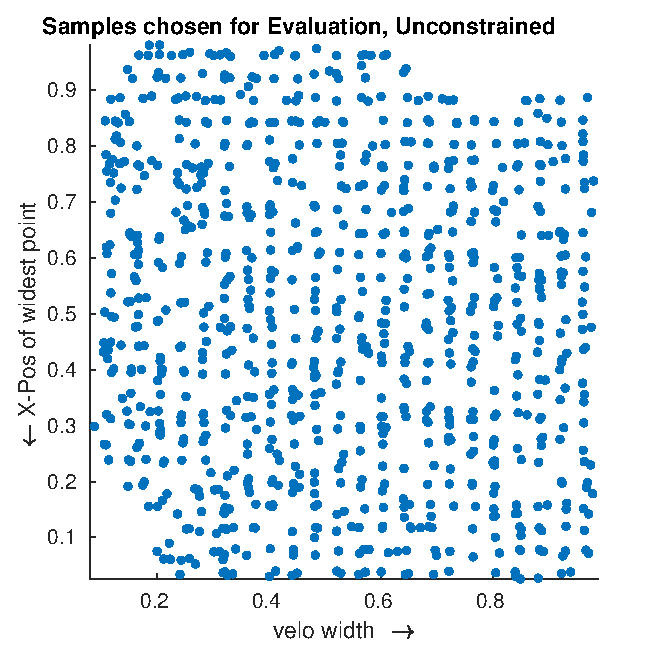
\includegraphics[width=1\linewidth]{bilder/6pt1000Samples/acqSamplesUncon}
		\caption{Kategorisierung der Samples, die für präzise Evaluationen ausgewählt wurden (ohne Constraint)}
		\label{fig:acqSamplesUncon}
	\end{minipage}\hfill
	\begin{minipage}{0.45\textwidth}
		\centering
		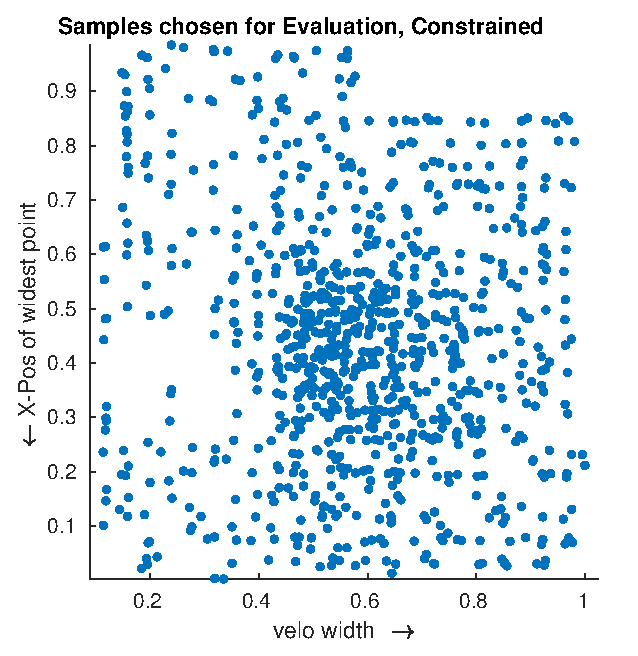
\includegraphics[width=1\linewidth]{bilder/6pt1000Samples/acqSamplesCon}
		\caption{Kategorisierung der Samples, die für präzise Evaluationen ausgewählt wurden (mit Constraint)}
		\label{fig:acqSamplesCon}
	\end{minipage}
\end{figure}

In \cref{fig:acqSamplesUncon,fig:acqSamplesCon} sind die phänotypischen Einordnungen der Individuen, die mithilfe der Akquisekarte zur Auswertung ermittelt wurden, für die Variante ohne und mit Constraint dargestellt.
Die Dimensionen sind dieselben wie in den vorigen Karten.
Zuerst ist zu beiden Varianten zu sagen, dass diese den Problemraum weitestgehend abdecken.
Einzig in der obere rechten und der unteren linke Ecke scheint weniger Exploration stattzufinden.
Abgesehen von diesen beiden Bereichen wird der Problemraum allerdings gut abgedeckt.
Interessant ist allerdings, dass die Abdeckung des Problemraums in der Variante ohne Constraint wesentlich regelmäßiger ist, als in der Variante mit Constraint
Zwar existieren einige Stellen an denen in der Variante ohne Constraint viele Auswertungen nah beieinander liegen, vor allem im linken Bereich des Graphen, insgesamt wird der Problemraum aber ausreichend weit erkundet.

Im Gegensatz dazu ist eine große Häufung an Akquiseindividuen im mittigen Bereich in der Version mit Constraint zu erkennen
und eine sehr geringe Konzentration an Akquiseindiviuen im linken Bereich bei $0,2 \leq x \leq 0,4$.
Dies ist besonders interessant dadurch, dass gerade der Bereich $0,2 \leq x \leq 0,4$ der ist, in dem die aerodynamisch besten Individuen liegen.
Durch die Einführung des Constraints, der effektiv eine Manipulation des Mittelwerts von UCB darstellt, wird der Bereich in dem Exploitation stattfindet dorthin verschoben, wo dieser Constraint besser erfüllt ist.
Dies ist grundsätzlich so gewollt, die Anhäufung von Punkten im mittleren Bereich kann allerdings ein Zeichen dafür sein, dass der Constraint im Vergleich zum Luftwiderstand zu stark gewichtet ist.
Gegebenenfalls wäre es sinnvoll den Constraint schwächer zu gewichten oder in der Akquisefunktion vollkommen wegzulassen und nur in der finalen Auswertung mit MAP-Elites zu betrachten.

\newcommand{\wheelcasepheno}[1]{
	\begin{figure}[h]
		\centering
		\begin{subfigure}[t]{0.5\textwidth}
			\centering
			\includegraphics[width=1\linewidth]{bilder/6pt1000Samples/#1-uncon-top.png}
			\subcaption{oben, ohne Constraint}
%			\label{fig:wheelcasepheno#1-uncon-front}
		\end{subfigure}\hfill
		\begin{subfigure}[t]{0.5\textwidth}
			\centering
			\includegraphics[width=1\linewidth]{bilder/6pt1000Samples/#1-uncon-angled.png}
			\subcaption{perspektivisch, ohne Constraint}
%			\label{fig:wheelcasepheno#1-uncon-angled}
		\end{subfigure}
		\begin{subfigure}[b]{0.5\textwidth}
			\centering
			\includegraphics[width=1\linewidth]{bilder/6pt1000Samples/#1-con-top.png}
			\subcaption{oben, mit Constraint}
%			\label{fig:wheelcasepheno#1-con-front}
		\end{subfigure}\hfill
		\begin{subfigure}[b]{0.5\textwidth}
			\centering
			\includegraphics[width=1\linewidth]{bilder/6pt1000Samples/#1-con-angled.png}
			\subcaption{perspektivisch, mit Constraint}
%			\label{fig:wheelcasepheno#1-con-angled}
		\end{subfigure}
		\caption{Die Phänotypen des Individuums (#1) mit und ohne Constraint}
		\label{wheelcasepheno#1}
	\end{figure}
}

\newcommand{\wref}[1]{
	\cref{fig:wheelcasepheno#1}
}

%\newcommand{\allrefWheelcase}[1]{
%	\cref{\wref{#1}{uncon-top},\wref{#1}{uncon-angled},\wref{#1}{con-top},\wref{#1}{con-angled}}
%}

Im Folgenden werden die Phänotypen einiger Individuen betrachtet und jeweils die Lösung der Zelle der beiden Versionen verglichen.
In den folgenden Abbildungen sind jeweils die Draufsicht sowie eine perspektivische Sicht auf den rechten Radkasten abgebildet.
Neben dem Velomobil ist auch das modellierte Constraintvolumen dargestellt und zur Differenzierung rot hervorgehoben.

\wheelcasepheno{4-2}

In \wref{4-2} sind die von MAP-Elites gefundenen Lösungen der Zelle (4-2) beider Versionen abgebildet.
Lösungen in dieser Zelle sind schmal, haben allerdings einen weit vorne liegenden breitesten Punkt.
Es ist ersichtlich, dass dies der Fall ist.
Es ist allerdings auch erkennbar, dass der Constraint in beiden Versionen nicht nur nicht erfüllt wird, sondern sogar sehr stark verletzt wird.
Es findet zwar eine klare Verbesserung des Constraints statt, wenn dieser explizit behandelt wird, der gewünschte Effekt, dass dieser aber vollkommen erfüllt wird ist hier nicht erreicht worden.
Dies hängt einerseits mit der Kategorisierung zusammen. Aus den beiden Draufsichten ist klar erkennbar, dass ein so schmales Velomobil den Constraint nie vollständig erfüllen kann.
Trotzdem interessant ist die Tatsache, dass die Variante mit Constraint nicht die maximal mögliche Constrainterfüllung aufweist, die bei der Breite möglich ist.
Stattdessen gehören beide Lösungen zur gleichen Lösungsklasse, die durch eine breitere Oberseite aber schmalere Unterseite charakterisiert wird.
Dass die Lösung, die in der Variante mit Constraint generiert wird, die physikalisch maximal möglich Constrainterfüllung nicht erlaubt, ist dadurch zu begründen, dass Constraint und Luftwiderstand gegeneinander gewichtet werden.
Die in der Variante ohne Constraint generierte Lösung stellt hierbei die in dieser Zelle optimale Lösung da.
Ein Abweichen von dieser Form muss jede Verschlechterung der aerodynamischen Eigenschaften durch eine Verbesserung des Constraint aufwiegen.
Dadurch entsteht aber das Problem der Gewichtung der beiden Ziele gegeneinander, welches enorm schwer zu lösen ist.
Will man Lösungen generieren, die den Constraint so gut wie möglich erfüllen unabhängig der damit verbundenen Kosten in der Aerodynamik, oder will man einen Kompromiss, wie er hier generiert wurde finden.
Wenn man einen Kompromiss finden will, muss man sich die Frage stellen, wo dieser liegen soll, bei einer 1:1-Gewichtung wie hier oder beispielsweise bei eine 2:1-Gewichtung.


\wheelcasepheno{4-25}

In \wref{4-25} sind schmale Velomobile, deren breitester Punkt im Gegensatz zum vorherigen Beispiel weit hinten liegt, dargestellt.
Trotzdem sind viele der in \wref{4-2} bereits beobachteten Tendenzen auch hier zu finden.
In beiden Varianten wird der Constraint auch hier nicht erfüllt.
Es ist zwar auch hier eine leichte Verbesserung zu erkennen, diese ist aber eher gering.
Besonders dadurch, dass die schmalen Velomobile den Constraint in der Variante ohne Constraint so stark verletzen lässt eigentlich viel Raum für Verbesserung, der offensichtlich nicht genutzt wird.
Dies ist hängt genau wie im vorigen Beispiel mit der Gewichtung zwischen Luftwiderstand und Constraint zusammen, durch die nur geringfügige Verbesserungen ermöglicht werden.
Auch ist interessant, dass dieser Phänotyp genau wie der im ersten Beispiel oben breiter und unten schmaler ist.


%\wheelcasepheno{25-1}

\wheelcasepheno{25-22}

In \wref{25-22} ist ein Individuum des anderen Extremes dargestellt.
Der dargestellte Phänotyp ist sehr breit und dessen breitester Punkt liegt weit hinten.
Es ist zu erkennen, dass der Constraint bereits in der Variante ohne Constraint recht gut erfüllt ist.
Dies deckt sich mit den Beobachtungen aus der Karte.
Da der Constraint in der Variante ohne Constraint bereits gut erfüllt ist, ist hier nicht viel potenzielle Verbesserung möglich.
Trotzdem findet eine Verbesserung statt und in der Variante mit Constraint ragt nur nach minimal aus dem Radkasten heraus.
Es ist interessant zu beobachten, dass diese Lösung einer anderen Lösungsklasse angehört als die beiden schmalen betrachteten.
Diese Lösung ist unten breiter und oben schmaler, es ist also ersichtlich, dass nicht nur dieselben Lösungen mit stärkeren und schwächeren Deformationen erzeugt werden.
Trotzdem stellen diese breiten Phänotypen aerodynamisch suboptimale Lösungen dar, gerade hier ist die Erzeugung von Lösungen zwar einfach aber eher uninteressant.
Das Ziel wäre schmalere Lösungen zu generieren die sowohl aerodynamische als auch Constraintoptimalität aufweisen.

\wheelcasepheno{12-12}

Alle vorigen Individuen befanden sich an den Rändern der Karte und stellten damit Extrema dar, zum Verständnis sollten sich daneben allerdings auch zentraler gelegene Individuen angeschaut werden.
In \wref{12-12} sind zwei solcher weniger extremen Individuen abgebildet.
Die größte Sache, die im Vergleich zu den vorher betrachteten Individuen auffällt, ist die signifikante Änderung bezüglich des Constraints.
Sowohl bei sehr schmalen als auch bei sehr breiten Individuen waren nur relativ kleine Änderungen bezüglich des Constraints zu erkennen.
Bei schmaleren Velomobilen lag dies daran, dass die geringe Breite eine vollständige Constrainterfüllung nicht zulässt und dass die Gewichtung zwischen Aerodynamik und Constraint so gewählt wurde, dass keine weiteren Verschlechterungen der Aerodynamik für Constraintgewinne in Kauf genommen wurden.
Bei breiten Velomobilen war der Constraint in der Variante ohne Constraint bereits weitestgehend erfüllt, wodurch keine signifikante Verbesserung durch die Einführung eines Constraints erreicht werden konnte.

Beide dieser Dinge gelten nicht für ein ausgeglichenes Individuum.
In der Variante ohne Constraint ist dieser offensichtlich nicht erfüllt.
Die Verbesserung in der Variante mit Constraint ist allerdings wesentlich signifikanter.
Der Constraint ist in dieser Variante bereits nahezu erfüllt, es sind noch zwei leichte Bänder auszumachen, in denen das Constraintvolumen aus dem Velomobil ragt, allerdings sind diese sehr klein.
Interessant ist auch der Unterschied zwischen der Lösungsklassen.
Während in der Variante ohne Constraint noch eine unten breitere oben schmalere Form präferiert wird -- Im Gegensatz zu dem bei schmaleren Lösungen präferierten Form, die oben breiter und unten schmaler war -- ist die Form in der Variante mit Constraint wesentlich gleichmäßig breiter.
Dies gilt in der Vertikalen, in der sowohl der untere Teil des Radkastens als auch der obere Teil breit sind, aber auch in der Horizontalen, in der der Radkasten wesentlich länger breit bleibt.

Was sich aus den betrachteten Phänotypen ablesen lässt ist, dass der Constraint überall beachtet wird und sich verbessert oder zumindest nicht verschlechtert.
Bei besonders breiten Velomobilen konnten keine signifikanten Verbesserungen erreicht werden, da der Constraint bei solchen breiten Lösungen meist schon fast vollständig erfüllt ist.
Hauptgewinne bezüglich des Constraints konnten bei zentraler Individuen gesehen werden, besonders bezüglich der Breite.
Bei schmaleren Individuen wurden die Constraintgewinne schmaler was auf eine Kombination aus Konflikt zwischen Aerodynamik und Constraint und in der Tatsache, dass constrainterfüllende Individuen schwerer zu generieren sind, je schmaler diese sein sollen.



%\subsubsection{Zusammenfassung}
%
%\todo[inline]{Alle drei Experimente, Trends unterschiede etc.}

\subsection{E-Roller}

\begin{table}[h]
	\centering
	\begin{tabularx}{.75\textwidth}{ll}\hline
		Anzahl initialer Samples & 60 \\
		%\rowcolor{lightgray}
		Anzahl Samples & 500 \\
		Anzahl neuer Samples pro Akquiseschleife & 10 \\
		%\rowcolor{lightgray}
		Anzahl Generationen Akquise-MAP-Elites & 2048 \\
		Kinder pro Generation Akquise-MAP-Elites & 32 \\
		%\rowcolor{lightgray}
		Anzahl Generationen Ergebnis-MAP-Elites & 4096 \\
		Kinder pro Generation Akquise-MAP-Elites & 32 \\
		Auflösung der MAP-Elites Karte & 25 * 25  \\
		\hline
		Freiheitsgrade & 20 \\
		Mittelwertgewichtung & 1 \\
		Varianzgewichtung & 2 \\
	\end{tabularx}
	\label{tab:parmasEscooter}
	\caption{Parametrisierung des E-Roller Experiments}
\end{table}



\begin{figure}[h]
	\centering
	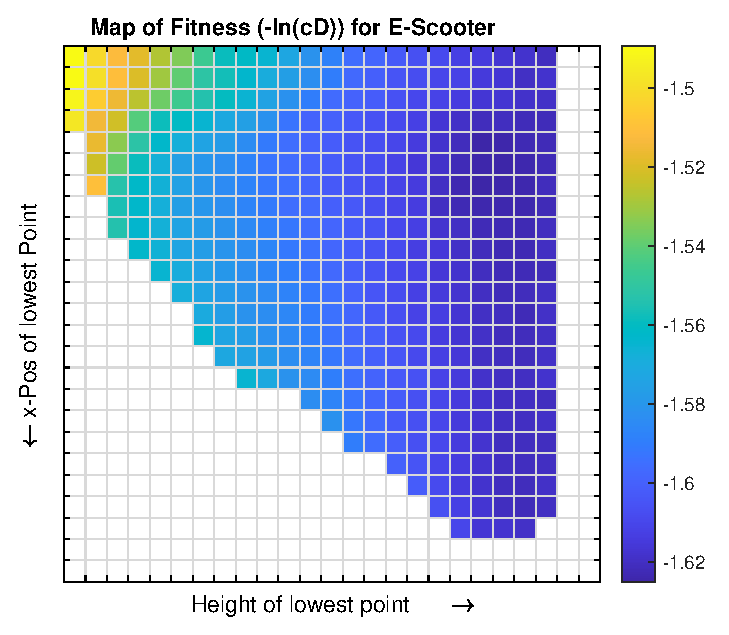
\includegraphics[width=.7\linewidth]{bilder/escooter/dragMapEscooter}
	\caption{Karte der Luftwiderstandswerte der E-Roller Domäne}
	\label{fig:dragMapEscooter}
\end{figure}

In \cref{fig:dragMapEscooter} ist die von SAIL für die E-Roller-Domäne produzierte Karte abgebildet.
Es ist erkennbar, dass die berechneten Fitnesswerte einen erstaunlich großen Bereich abdecken, dafür, dass nur ein eher kleines Bauteil an der Unterseite des E-Rollers deformiert wird.
Aufgrund der oben erwähnten Einschränkung bezüglich der Ergebnisse, sollte dies nicht als Zeichen gedeutet werden, dass Deformationen in diesem Bauteil tatsächlich so große Änderungen bewirken können.
Dass solche signifikante Änderungen existieren ist zur Anwendung von SAIL allerdings gut, sind die Variationen zwischen Individuen zu gering kann SAIL nicht korrekt arbeiten, da der als Surrogatmodell genutzte Gaußprozess auf solchen Daten nur schlecht trainiert werden kann.
Der Gradient der auf den generierten Daten erkennbar ist lässt allerdings auch darauf schließen, dass die Ergebnisse von Openfoam nicht zu stark Rauschen.
Wäre alle Varianz der Ergebnisse von Openfoam bloß auf Rauschen zurückzuführen, wäre es nicht zu erwarten, dass eine Karte mit einem relativ glatten Gradienten erzeugt wird.
\begin{table}[h]
	\centering
	\begin{tabularx}{.25\textwidth}{ll}\hline
		$\ell$ & 2,2791 \\
		$\sigma_f$ & 0,0473 \\
		$c$ & -1,4904 \\
		$\sigma_n$ & 0,0114 \\
	\end{tabularx}
	\label{tab:hyperparamsEscooter}
	\caption{Die Hyperparameter des Gaußprozesses nach Anpassung}
\end{table}
Diese Tatsache kann auch an den Hyperparametern, die für die E-Roller-Daten optimiert, werden abgelesen werden.
Diese sind in \cref{tab:hyperparamsEscooter} aufgeführt.
Das benötigte Signalrauschen, welches von der Optimierungsfunktion berechnet wird um die Daten ausreichend beschreiben zu können beträgt $0,0114$, und ist damit ungefähr zehnmal kleiner als die Reichweite der Lösungen in der Karte.
Aus diesen Beobachtungen kann geschlossen werden, dass die Ergebnisse der Openfoam-Simulation zumindest ausreichen um SAIL mit diesen durchführen zu können.
Dies sagt selbstverständlich nichts über die Korrektheit der Openfoam-Simulation aus nur, dass die vorliegenden Daten von ihren qualitativen Eigenschaften für SAIL geeignet sind.

Auch die sonstigen Hyperparameter des Gaußprozesses liegen in plausiblen Größenordnungen.
Der Mittelwert von $-1,49$ liegt sehr exakt bei den in der Karte dargestellten Werten.
Ein Längenmaß von $\ell=2,28$ ist zwar eher groß, problematischer wäre es allerdings, wenn dieses zu klein wäre.
Ein typisches Zeichen von einem zu groß gewählten Längenmaß ist, dass starkes Rauschen benötigt wird, um die Daten zu erklären.
Da das Rauschen, durch $\sigma_n$ bestimmt, allerdings relativ klein ist, ist ein solches Längenmaß nicht außergewöhnlich.

Unter der Annahme, das die Werte aus den Openfoam-Simulationen ausreichen präzise sind, lassen sich einige Dinge aus der Karte ablesen.
Das erste ist der Gradient in der Horizontalen.
Lösungen deren tiefster Punkt tiefer liegt weisen schlechtere Luftwiderstandskoeffizienten auf als solche, die flacher sind.
Die zweite Sache die in der Horizontalen auffällt, ist der strenge Abriss von Lösungen nach der 23ten Spalte.
Dies ist durch die Auswahl der ersten Kategorie zu erklären.
So ändert sich der tiefste Punkt für Deformationen nach unten, und wird meist einer der deformierten Punkte sein.
Für Deformationen nach oben gilt dies nicht, stattdessen wird dort ein Punk am Rand der FFD-Box zum tiefsten Punkt, der unabhängig von der Stärke der Deformation immer der tiefste Punkt bleiben wird.
Alle Bauteile, die entweder sehr flach sind oder nach oben deformiert werden, werden also in die rechteste Befüllt Spalte eingeordnet, da es mit der momentanen FFD-Konfiguration nicht möglich ist Individuen Bauteile zu generieren, deren tiefster Punkt höher liegt.
Entlang der anderen Dimension ist kein so starker Effekt zu beobachten, hier fallen allerdings zwei Dinge auf.
Hier scheint eine Optimum, etwa in der fünften Zeile, zu existieren.
Sowohl Lösungen deren tiefster Punkt weiter vorne liegt, als auch solche, deren tiefster Punkt weiter hinten liegt besitzen leicht schlechtere Luftwiderstandswerte.
Die zweite auffällige Eigenschaft in der Vertikalen ist, dass die Anzahl an Lösungen pro Spalte nicht vergleichbar ist, sondern zunimmt, je höher der tiefste Punkt der Bauteile der Spalte liegt.
Dies ist durchaus interessant, da die momentanen Deformationspunkte grundsätzlich in der Lage sein sollten einen tiefsten Punkt weiter vorne zu generieren.
\todo{warum trotzdem?}

\begin{figure}[h]
	\centering
	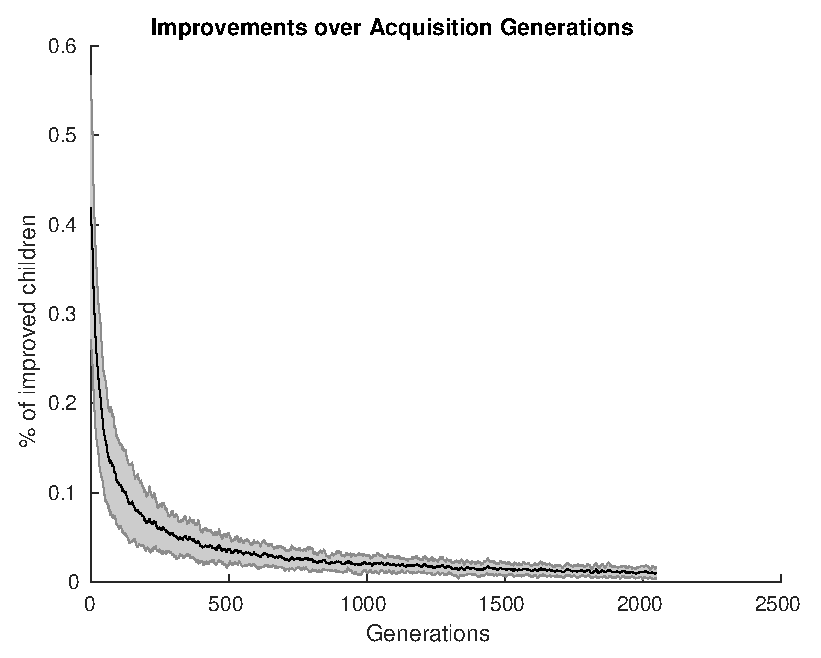
\includegraphics[width=.7\linewidth]{bilder/escooter/acqImprovements}
	\caption{Prozentuale Verbesserung der Kinder pro Akquisegeneration}
	\label{fig:escooteracqImprovement}
\end{figure}

In \cref{fig:escooteracqImprovement} ist die prozentuale Verbesserung über die Akquisegenerationen abgebildet.
Auch diese sieht so weit nicht uncharakteristisch aus.
Es werden Verbesserungen zu Lösungen gefunden und über die Generationen konvergiert die Anzahl an Verbesserungen immer stärker, wodurch die charakteristische logarithmische Form entsteht.

\newcommand{\escooterpheno}[1]{
\begin{figure}[h]
	\centering
	\begin{subfigure}[t]{0.5\textwidth}
		\centering
		\includegraphics[width=1\linewidth]{bilder/escooter/#1-front.png}
		\subcaption{vorne}
%		\label{fig:escooterpheno#1-front}
	\end{subfigure}\hfill
	\begin{subfigure}[t]{0.5\textwidth}
		\centering
		\includegraphics[width=1\linewidth]{bilder/escooter/#1-side.png}
		\subcaption{Seite}
%		\label{fig:escooterpheno#1-side}
	\end{subfigure}
\caption{Die Phänotypen des Individuums (#1)}
\label{fig:escooterpheno#1}
\end{figure}
}

\newcommand{\escref}[1]{
	\cref{fig:escooterpheno#1}
}

\escooterpheno{1-1}

In \escref{1-1} (a) ist der Phänotyp des ersten Individuums in der ersten Spalte von vorne dargestellt.
In \escref{1-1} (b) ist derselbe Phänotyp von der Seite dargestellt.
Individuen der ersten Spalte zeichnet aus, dass deren tiefster Punkt besonders tief ist.
Individuen der ersten Zeile zeichnet aus, dass deren tiefster Punkt weiter hinten liegt.
Es ist sehr klar erkennbar, dass der dargestellte Phänotyp diese Kategorien erfüllt.


\escooterpheno{23-22}

Der Phänotyp in Zelle (23,22)(3. Spalte von links, 4. Zeile von unten) dargestellt in \escref{23-22} stellt das Gegenteil des vorigen Phänotyps dar.
Dessen tiefster Punkt sollte besonders weit oben und eher vorne liegen.
Insgesamt ergibt sich dadurch eine sehr flache Form, deren tiefster Punkt weit vorne liegt und die sogar leicht das Gestänge der Radhalterung schneidet.

\escooterpheno{9-16}

Das dritte Beispiel ist im Gegensatz zu den vorigen beiden keines der Extrema, sondern ein Individuum aus dem mittigen Bereich der Karte.
Das Individuum (9,16) dargestellt in \escref{23-22} befindet sich am Dreiecksrand der Karte.
Dieses Individuum ist nicht so schlecht wie das erste ausgewählte Individuum, bietet aber trotzdem eine interessantere deformierte Form als das untere rechte Individuum.
Es ist klar erkenntlich, dass eine Deformation nach unten stattfindet, diese aber wesentlich schwächer ausfällt als im ersten Beispielindividuum.
Sehr interessant ist auch, dass das Individuum (9-16) nach hinten wieder abflacht beziehungsweise geschlossen ist.
Dies steht im Gegensatz zum ersten Beispielindividuum, welches nach hinten geöffnet war.
Das bedeutet, dass das Ziel von SAIL nicht nur morphologisch unterschiedliche Lösungen derselben Lösungsklasse zu generieren, sondern eine Diversität an Lösungsklassen zu generieren teilweise erfüllt wird.

\escooterpheno{20-5}

Das letzte Beispiel, dessen Phänotyp genauer angeschaut wird liegt im letzten Bereich der Karte auf den bisher noch kein Blick geworfen wurde, der oberen rechten Ecke.
In \escref{20-5} ist das Individuum (20,5) abgebildet, welches nicht das extremste Individuum der rechten Ecke ist, sondern, das welches den optimalen Fitnesswert aufweist.
Es ist herauszustellen wie ähnlich dieses Individuum dem Individuum (23,22) ist.
Zwar liegt der tiefste Punkt weiter hinten, da beide Individuen allerdings sehr flach sind, ändert die Position des tiefsten Punkts, der nur leicht unter dem restlichen Bauteil liegt, die Form nicht signifikant.
Dadurch fallen beide in die gleiche Lösungsklasse.

Dies zeigt eine Problematik der gewählten Kategorien auf.
Da die Position des tiefsten Punktes bei einer Platte keinen wirklichen Einfluss auf den erzeugten Phänotypen hat, werden hier am rechten Rand eine Reihe von Lösungen entwickelt, die am Ende keine wirkliche phänotypische Diversität aufweisen.
Dies bezieht sich zwar nur auf den rechten Rand und weiter links entstehen signifikante phänotypische Unterschiede zwischen Individuen in einer Spalte, allerdings sind die Spalten, weiter links in der Karte immer spärlicher gefüllt.
Das heißt, sowohl zum linken Rand als auch zum rechten Rand der Karte nimmt die Diversität der Spalten aus unterschiedlichen Gründen ab.
Das ist ein klares Indiz, dafür, dass die x-Position des tiefsten Punktes keine gute Kategorie darstellt und vermutlich durch eine andere Kategorie, die in der Lage ist, mehr Diversität zu erzeugen ausgetauscht werden sollte.
Auch ist die Anzahl an verschiedenen Lösungsklassen gering. Die Lösungen lassen sich hauptsächlich in nach hinten offene, nach hinten geschlossene und flache Lösungen aufteilen.

Zudem ist interessant, dass die generierten Lösungen alle fast symmetrisch sind.
Die Lösungen sind so nah an einer symmetrischen Lösung, dass die Asymmetrie nicht auf einen expliziten Vorteil dieser hindeutet, sondern dass die Erzeugung perfekter symmetrischer Bauteile bei 20 Freiheitsgraden aufwendig für den evolutionären Algorithmus ist und deshalb nur fast symmetrische Bauteile entstehen.
Besonders in Anbetracht der Tatsache wie viele asymmetrische Lösungen theoretisch möglich sind, stellt die Erzeugung von nur praktisch symmetrischen Teilen einen Trend dar.
Das war zwar grundsätzlich zu erwarten, da der E-Roller symmetrisch ist und damit die Erwartung besteht, dass Strömungen um diesen auch symmetrisch sind.
In solchen Strömungen wären Bauteile die symmetrisch sind erwartungsgemäß optimal. 
Die Ergebnisse bestätigen diese Erwartungen weites gehend.

\begin{figure}[h]
	\centering
	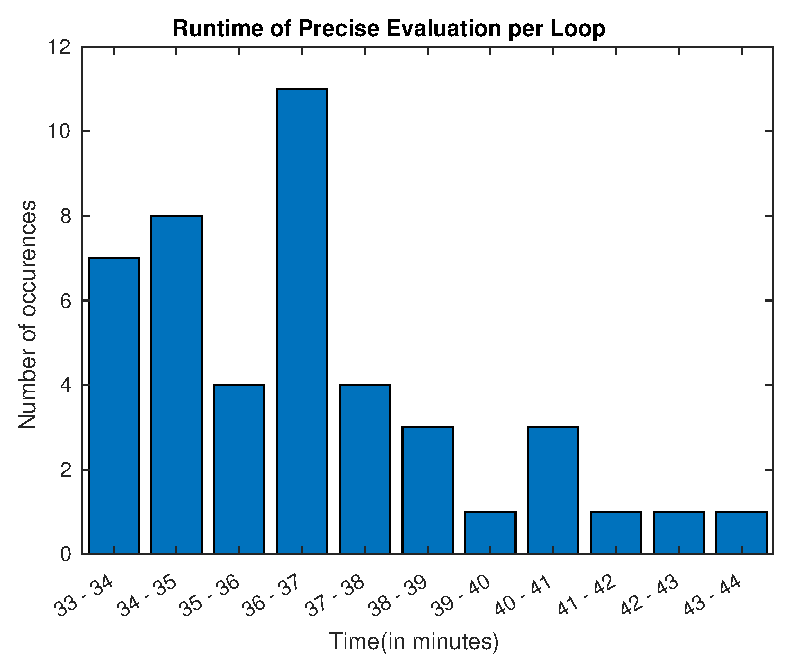
\includegraphics[width=.7\linewidth]{bilder/escooter/peRuntime}
	\caption{Laufzeiten zur parallelen Evaluation von 10 präzisen Evaluationen}
	\label{fig:escooterpeRuntime}
\end{figure}

Ein nicht unwichtiger Teil in der E-Roller-Domäne, der zwar nur indirekt etwas mit SAIL zu tun hat, sind die Openfoam-Simulationen.
Besonders auffällig war, dass diese in der E-Roller-Domäne wesentlich rechenaufwendiger ausfielen.
In \cref{fig:escooterpeRuntime} sind die Laufzeiten der präzisen Auswertungen pro Schleifeniteration dargestellt.
Insgesamt wurden in jeder der 44 Schleifeniterationen 10 Individuen\footnote{500 Gesamtsamples - 60 Initialsamples = 440 Akquisesamples} parallel ausgewertet.
Die dargestellten Zeiten sind nicht nur die für die Openfoam, sprich Zerlegung snappyHexMesh, Simulation etc., benötigten Zeiten, sondern beinhalten einen Overhead von Matlab, wie die Datenverteilung auf 10 Worker und die Fitnessberechnung.
Nichtsdestotrotz stellen die Openfoam-Funktionen den größten Teil des Zeitbedarfs dar.
Die beträchtliche Laufzeit, die für Openfoam benötigt wird erzeugt eine Obergrenze an präzisen Funktionsauswertungen die durchgeführt werden können.
Ein großer Teil der Laufzeit ist auf die 1000 simulierten Sekunden zurückzuführen.
Eine Analyse der Darstellung durch Openfoam sollte aber neben einer qualitativen Untersuchung der Korrektheit der Simulation auch eine Untersuchung der Laufzeit umfangen.
Die Verbesserung der Laufzeit ist durch unterschiedliche Methoden möglich.
Kann eine Openfoamparametrisierung gefunden werden in der die cD-Werte schneller konvergieren, könnte die simulierte Dauer vermindert werden.
Es könnte unnötiger File-I/O in Openfoam minimiert werden und die Dekomposition zur parallelen Bearbeitung der Cases analysiert werden.
Zuletzt wäre eine Analyse welche Teile des E-Rollers einen signifikanten Einfluss auf die Strömung um das Bauteil habe und welche das nicht haben und folglich ohne Präzisionsverlust wegrationalisiert werden können angebracht.


%\begin{figure}
%	\begin{tabularx}{.75\textwidth}{ll}\hline
%		Anzahl initialer Samples &  \\
%		Anzahl Samples &  \\
%		Anzahl neuer Samples pro Akquiseschleife & \\
%		Anzahl Generationen Akquise-MAP-Elites & \\
%		Kinder pro Generation Akquise-MAP-Elites & \\
%		Anzahl Generationen Ergebnis-MAP-Elites & \\
%		Kinder pro Generation Akquise-MAP-Elites &  \\
%		Auflösung der MAP-Elites Karte &   \\
%		\hline
%		Freiheitsgrade &  \\
%		Mittelwertgewichtung & 1 \\
%		Varianzgewichtung & 2 \\
%		Constraintgewichtung & 1 \\
%	\end{tabularx}
%\end{figure}
